% In this section, we present our algorithm for computing the upper bound for a program $c$'s adaptivity
% $A(c)$ defined~\ref{def:trace_adapt} through static program analysis.
% This section presents the key definitions
% for the static analysis algorithm in Section~\ref{sec:algorithm-keys} before going into the detail of the algorithm,
% then shows the complete static analysis algorithm.
% \mg{
% In this section, we present our static program analysis for computing an upper bound on the adaptivity a program $c$
% }
In this section, we present our static program analysis algorithm for computing 
% an upper bound on the 
% execution-based reachability times 
the \emph{reachability-bound} for every program point $l$ in a program $c$ in a path sensitive manner.
% , as defined in last section.
%
\subsection{Algorithm Overview}
\label{sec:alg_overview}
% In order to have the upper bound of the reachability for every label of a program $c$, we design 
% a path sensitive reachability bound analysis algorithm {\THESYSTEM}.
The algorithm is summarized into the following steps,
% \begin{figure}
%   \centering    
% 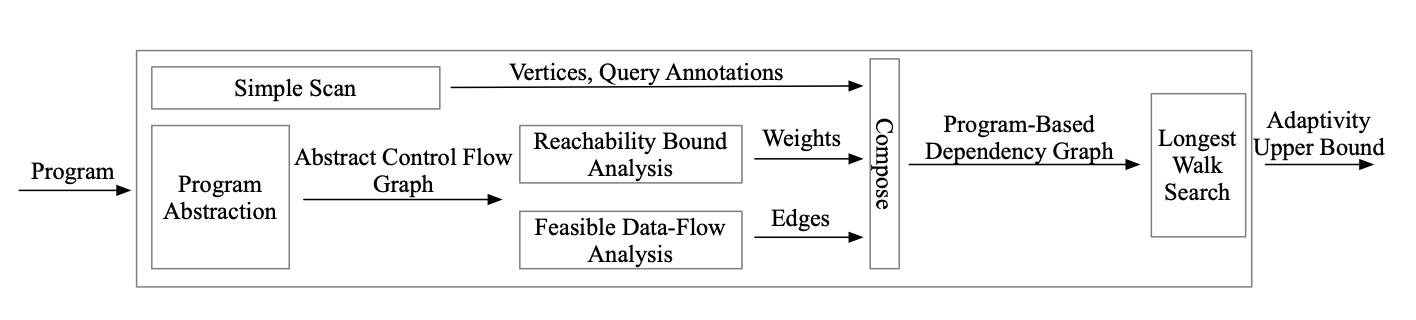
\includegraphics[width=1.0\columnwidth]{adapfun.png}
%   \vspace{-0.3cm}
%   \caption{The overview of {\THESYSTEM}}
%   \label{fig:adaptfun}
%   \vspace{-0.5cm}
% \end{figure}
%
%
\begin{enumerate}
\item  In Section~\ref{sec:abs_prog}, we first construct an abstract transition graph based on $c$, by computing an abstract transition 
for every labeled command. 
This graph is used in the following sections
%  from Section~\ref{sec:refine} to Section~\ref{sec:psrbcompute} 
for computing the path-sensitive reachability-bound of a program location.
% see Section~\ref{sec:alg_vertexgen}
\item Section~\ref{sec:refine}
refines the multiple-paths loops in the program
% this program path sensitively, 
based on the abstract transition graph.
This step transforms the multiple-paths loops into multiple loops where
the interleaving of paths is explicit.
%  which come from its abstract transition graph.
\item Section~\ref{sec:lbcompute} computes the ranking function  
\footnote{\textbf{ranking function} is the named used in \cite{SinnZV14}
and \textbf{local bound} is the name used in \cite{ZulegerGSV11}, \cite{SinnZV17}.
We refer to the two names as the same meaning in this paper.} for each edge in a program's abstract transition graph,
and estimates the upper bounds on every ranking function's maximum value and every edge's execution times path-insensitively.
% path-insensitive reachability upper bound for every while loop command in $c$.
\item Section~\ref{sec:outinalg} performs the \textbf{Outside-In} algorithm and computes
the upper bound for the execution times of \todo{certain sub-sequence} of paths in a refined program locally, named \textbf{Outside-In} bound.
% path-sensitive local bounds.
\item Section~\ref{sec:inoutalg} performs the \textbf{Inside-Out} algorithm and 
computes the upper bound for the execution times of
every distinct path in a refined program globally, named \textbf{Inside-Out} bound.
% abstract transition graph.
\item Section~\ref{sec:psrbcompute} computes the path-sensitive reachability-bound for every program point
%  in this program 
based on the above results.
%  by
%  ?summarizing 
% the path-sensitive reachabilitybound of each edge on the abstract transition graph.
% \item The Section~\ref{sec:reachabilitybound_algorithm} computes program's reachability bound in two steps as follows.
\end{enumerate}
% Finally, with all the ingredients ready, we construct the final approximated program-based dependency graph in Section~\ref{sec:alg_graphgen}
% the algorithm  without extra static analysis technique.
% \\
% Overall, this program-based graph has a similar topology structure as 
% % the one
% % of 
% the Execution-Based Dependency Graph. It has the same
% vertices and query annotations, but approximated edges and weights. We call the graph generated by static analysis techniques, static analysis dedendency graph. 
% \item Then in the last phase in Section~\ref{sec:alg_adaptcompute}, $\THESYSTEM$
% % we compute the upper bound for adaptivity over this approximated graph:
% % , as an upper bound for
% % program's adaptivity
% computes the upper bound for adaptivity over this approximated graph.
% in the last phase of this algorithm in Section~\ref{sec:alg_adaptcompute}.
% \subsection{Adaptivity Based on Program Analysis in \THESYSTEM}
% In order to give a bound on the program's adaptivity, we first build a
% program-based data-dependency graph to {over-}approximate the
% trace-based dependency graph.  Then, we define a program-based
% adaptivity over this approximated graph, as an upper bound for
% $A(c)$.
% %
% \subsection{ $\THESYSTEM$ Analysis Algorithm}
% \subsection{Dependency Graph Estimation}
% \subsection{Vertices Estimationn}
% \label{sec:alg_vertexgen}
% The first component of every vertex in the static analysis dependency graph are actually identical as the  Execution-Based Dependency Graph, which are assigned variables in the program annotated with the unique label(line number). 
% These vertices are collected by statically scanning the program, like what we do for vertices of its Execution-Based Dependency Graph. 
% The vertices are defined formally as follows.
%   \highlight{
% \[
%     \progV^0(c) \triangleq \left\{ 
%   (x^l, w) \in \mathcal{LV} \times \mathcal{A}_{\lin}
%   ~ \middle\vert ~
%   x^l \in \lvar(c)
%   \right\}
%   \]
%   }
%   %
% where $\mathcal{A}_{\lin}$ is the set of arithmetic expressions over $\mathbb{N}$ and program's input variables. 
% The weight $w$ for every vertex will be computed in following step in Section~\ref{sec:alg_weightgen}.
% The static scanning of the programs also tells us whether one vertice(assigned variable) is assigned by a query request. We have similar definition when defining the Execution-Based Dependency Graph, 
% a set of pairs $\progF(c) \in \mathcal{P}(\mathcal{LV} \times \{0, 1\} )$ 
% % is the set of pairs 
% % The weight for each vertex in $\progV(c)$ is computed 
% mapping each $x^l \in \progV(c)$ to a flag, either $0$ or $1$, where $1$  means $x^{l}$ is a member of $ \qvar_{c}$, a set of those variables assigned with query requests, and $0$ means $x^{l}$ not in this set. It is defined formally below.

% \[\progF(c) =\left\{(x^l, n)  \in  \mathcal{LV} \times \{0, 1\} 
% ~ \middle\vert ~
% x^l \in \lvar_{c},
% n = 1 \iff x^l \in \qvar_{c} \land n = 0 \iff  x^l \not\in \qvar_{c} .
% \right\}\]
%

% \wq{To do: Add $\THESYSTEM$, a data flow analysis algorithm to scan the program and give a graph.}
% {\THESYSTEM} consists of three phases: 
% \begin{enumerate}
%     \item Generating an abstract transition graph with each edge representing an abstract event transiting between two command labels. 
%     \item Computing the value bound invariant for each variable in the event and 
%     the event transition closure over the abstract transition graph,
%     we get the reachability bound for each labeled command.
%     \item Refining the abstract transition graph with data-flow, by performing the reaching definition analysis, we generate a weighted data control flow graph.
%     \item An algorithm to find the appropriate path in the weighted data control flow graph
% \end{enumerate}

% \begin{enumerate}
%     \item An algorithm to generate a precise data control flow graph
%     \item An algorithm to perform a Reachability number analysis to calculate the weight of each node in the graph generated in phase 1.
%     \item An algorithm to find the appropriate path in the weighted data control flow graph
% \end{enumerate}

% \subsection{Edge and Weight Estimation}
% \label{sec:alg_weightedgegen}

% Since the edges of the execution-based graph of a program relies on the dependency relation, which handles both control flow and data flow, as an over-approximation of this graph, the edges of our static anlaysis dependency graph also covers these two kind of flows. We develop a feasible data flow relation to catch these two flows, in Section~\ref{sec:alg_edgegen}.


% The weight of every vertice in the execution-based graph is built on all possible execution traces.
% In order to over-approximate the weight statically but still tightly, we present a symbolic reachability bound analysis for estimation of the weight of each vertice(label) in Section~\ref{sec:alg_weightgen},
% in spirit of some reachablility bound techiniques.


% The edges and weight estimation are both performed on basis of an abstract transition graph of the program, we first show how to generate this abstract transition graph before the introduction of  the edge and weight estimation.  

% This analysis first 
%  generate an abstract transition graph
%  over all program labels, 
% in order to analyzing the data flow relations through variables assigned in every labeled command,
% and the reaching time of each variable.
% Then, it refines this control flow graph 
% % into a weighted data-dependency graph, 
% and generate the Program-Based Dependency Graph,
% through the data flow and reaching bound analysis results.
% In the last step, it finds the longest finite walk in this weighted data control flow graph w.r.t. the query variables,
% and return the number of query vertices traversed alongside.
% % \wq{To do: Add $\THESYSTEM$, a data flow analysis algorithm to scan the program and give a graph.}
% To be more specific, {\THESYSTEM} consists of five phases as follows,
% \\
% % \jl{Better to have a graph or picture of overview of the algorithm}
% \todo{graph}
% \todo{pass again}
% This analysis
% \begin{enumerate}
%     % \item Generating 
%     \item first generate 
%     an abstract transition graph
%     %  over all labels,
%     (remove?? with program's labels as vertices and abstract transitions as edges)
%     in Section~\ref{sec:abs_prog},
%     % used to analyze 
%     for analyzing the weight of every vertex in $\progV(c)$ and edges between every vertex in $\progV(c)$ in the next two steps;
%     %  \ref{sec:alg_weightgen} and 
%     % \ref{sec:alg_edgegen}.

%     % which are used as program's program points,
%     %
%     \item then use the abstract transition graph generated above, 
%     compute the weight of every vertex in $\progV(c)$ by computing a symbolic reachability bound for each label in Section~\ref{sec:alg_weightgen},
%     % \\
%     \item and then use the same graph again to estimate the edges between every vertex in $\progV(c)$ by computing the feasible data flow relation between every labeled variables in Section~\ref{sec:alg_edgegen}.
  
% \end{enumerate}

\subsection{Abstract Transition Graph}
\label{sec:abs_prog}

This path-sensitive reachability-bound algorithm
is performed on basis of an \emph{Abstract Transition Graph} for the program $c$.
% We first show 
This step shows how to generate the abstract transition graph $\absG(c)$ of a
program $c$ through constructing its vertices and edges.
%  before the introduction of the edge and weight estimation.  
% We discuss the vertices and edge of the
% abstract transition graph for a program $c$, $\absG(c)$.

\subsubsection{Vertices Construction}
\label{sec:abs_prog-vertex}
Every 
vertex corresponds to a program execution point, which is a unique
label of a command in this program.
Specifically,
the vertices of this graph is the set of $c$'s labels with the exit label ${\lex}$, 
\[ 
  \absV(c) = \lvar(c)\cup\{{\lex}\}
  \]
%  corresponding to a label command in the program.

\subsubsection{Edge Construction}
\label{sec:abs_prog-edge}
  The vertices can be easily collected and the key point of the abstract
  transition graph for a program is constructing the edge set, $\absE(c)$ for a program $c$.
  It relies on the control flow analysis and the program abstraction of each command.
  %  and abstract transition (we also call it abstract event).
  To make it easy to understand, it
  is an enriched control flow graph with an annotation on each edge.
  The edge set is constructed by a program abstraction method in three steps.
  \\
  In the first step, \textbf{Constraint Computation} generates the constraint
  for the expression in each program command,
  which is used as the annotation of an edge.
  \\
  In the second step, \textbf{Initial and Final State Computation} generates two sets for each command. 
  The initial state is a set that contains the
  program point where this command \todo{starts} executing, 
  and the final state is a set
  that contains the constraint of this command
  and the continuation program points after the execution of this command.
  \\ 
  In the third step, \textbf{Abstract Event Computation} generates a set of edges for the program.
  Each edge is a pair of initial and finial state.
  % The annotation of each edge is a constraint generated by a program abstraction method.
  % by adopting the program abstraction.
  %  method in Section 6 in~\cite{SinnZV17}.
  %  the program's every command.
% It is computed as follows.
  % The edge in the abstract transition graph comes from the abstract execution trace of the program. 
  % The abstract execution trace, an abstract representation of the execution, consists of a set of abstract events. 
%   The edge in the abstract transition graph comes from the program's abstract events set $\absflow(c)$.
%   Each abstract event $(l_1, dc, l_2)$ in this set represents an edge in $\absE(c)$.
%   % Then, every abstract transition in the abstraction execution trace corresponds to an edge in the abstract transition graph. In another word, the edge $(l_1, dc, l_2)$ in the abstract transition graph, represents an abstract transition 
% %  from $l_1$ to $l_2$, with a set of difference constraints $dc$. 
%  Also notice, the difference constraints generated during the abstract transition appears in the edge as annotation.
%
\paragraph{Constraint Computation}
In this step, we first show how to compute the constraints for expressions in a program $c$,
by a program abstraction method adopted from the
algorithm in Section 6 in~\cite{SinnZV17}.
\\
Given a program $c$,
every arithmetic expression in an assignment command with label $l$,
or boolean expression in the guard of a $\eif$ or $\ewhile$ command with label $l$
is transformed into a constraint.
\\
This constraint describes the abstract execution of the assignment command with label $l$,
or abstract evaluation of the boolean expression in the guard with label $l$.

\highlight{Notations / Formal Definitions:}
\begin{itemize}
\item Operator: $\absexpr : \mathcal{A} \cup \mathcal{B} \to DC(\mathcal{VAR}  \cup \constdom)\cup \booldom \cup \{\top\}$
%
\item Constraints $\dcdom^{\top}: DC(\mathcal{VAR}  \cup \constdom) \cup \booldom\cup \{\top\}$  contains:
%
\begin{itemize}
\item Difference Constraints $DC(\mathcal{VAR}  \cup \constdom)$ is the set of all the inequality of
form $x' \leq y + v$ where $x \in \mathcal{VAR} $, 
$y \in \mathcal{VAR}$ and $v \in \constdom$.
The \emph{Symbolic Constant} set $\constdom = \mathbb{N} \cup \inpvar \cup{\infty}$
is the set of natural numbers with $\infty$ and input variables.
An inequality $x' \leq y + v$ describes that the value of $x$ in the current state is
at most the value of $y$ in the previous state plus some constant $v$.
$x' \leq y + v$ on an edge describes $l \xrightarrow{x' \leq y + v} l'$ describes
that after evaluating the assignment command with label $l$, the value of $x$ is
at most the value of $y$ before executing this command plus some constant $v$.
%
\item The Boolean Expressions $b$ from the set $\booldom$.
$b$ on an edge $l \xrightarrow{b} l'$ describes
that after evaluating the guard with label $l$,
$b$ holds and the command with label $l$ will execute right after.
%
\item The top constraint, $\top$ denotes always true. It is preserved for $\eskip$ command.
\end{itemize}
\end{itemize}

\highlight{Computation Steps:}
\begin{defn}[Constraint Computation]
  \label{def:constraint_compute}
  For a program $c$, a boolean expression $\bexpr$ in the guard of a $\eif$ or $\ewhile$ command
  or an expression $\expr$ and a variable $x$
  in an assignment command $\assign{x}{\expr}$,
  % or 
  % For a boolean expression $\bexpr$ or an arithmetic expression $\aexpr$ and a variable $x$,
  the constraint $\absexpr(\bexpr, \_)$ or $\absexpr(x - v, x)$ is computed as follows,
  \[
    \begin{array}{ll} 
      \absexpr(x - v, x)  = x' \leq x - v  & x \in \grdvar \land v \in \mathbb{N} \\
      \absexpr(y + v, x)  = x' \leq y + v  & x \in \grdvar \land v \in \mathbb{Z} \land y \in (\grdvar \cup \constdom) \\
      \absexpr(v, x)  = x' \leq v + 0  & x \in \grdvar \land v \in (\grdvar \cup \constdom) \\
      \absexpr(y + v, x)  = x' \leq y + v & \\
      \grdvar = \grdvar \cup \{y\} & x \in \grdvar \land v \in \mathbb{Z} \land y \notin (\grdvar \cup \constdom)  \\
      % \absexpr(\qexpr, x)  = x' \leq 0 + Q_m & x \in \grdvar \land \qexpr \text{ is a query expression}  \\
      \absexpr(\expr, x) = x' \leq \infty  &  x \in \grdvar \land \expr \text{ doesn't have any of the forms as above} \\
      \absexpr(\expr, x) = \etrue  &  x \notin \grdvar \\
      \absexpr(\bexpr, \_) = \bexpr   & \\
      % \absexpr(y + v, x)  = x' \leq y + v & \\
      \grdvar = \grdvar \cup FV(\bexpr) &  x \in \grdvar \land \bexpr \text{ is a boolean expression} \\
    \end{array}
    \]
  \end{defn}
%
  $\grdvar$ is the set of variables used in the guard expression of every while command in the program $c$. 
  In the case 4, if a variable $x$, belonging to the set 
  $\grdvar$ is updated by a variable $y$, which isn't in this set, 
  we add $y$ into the set $\grdvar$ and repeat 
  above procedure  until $\grdvar$ and $\absexpr(\expr, x)$ is stabilized. 
  % \wq{I do not understand this sentence:-(}
  \\
Specifically 
% understanding the intuition, 
we handle a 
% simplified 
normalized expression, $x > 0$
in guards of while loop headers, and 
%  \wq{I do not understand this sentence:-(}
%  .
% \\
% The counter variables only increase, decrease or reset by expression in the form of arithmetic minus and plus (able to extend to max and min.)
the counter variable $x$ only increase, decrease or reset by 
% expression in the form of 
simple arithmetic expression (mainly multiplication, division, minus and plus (able to extend to max and min)). 
The counter variable $x$ is generalized into norm when the boolean expression $x > 0$
in $\ewhile$ doesn't have the form $x > 0$.
The way of normalizing the guards and computing the norms is adopted from the computation step 1 in Section 6.1 in paper \cite{SinnZV17}. 
% \\
% For more complex expression assignments, where the counter reset, or calculated from $\elog$, 
% multiplication or division, and expressions involving multiple variables, the constraint is approximated as reset of $\infty$.
% \\
% % This simplification \wq{which part we simplify here?} 
% This approximation strategy
% doesn't affect our analysis results in our examples. It is easy to extend the normalized expression 
% into more complex forms as in \cite{SinnZV17}, as well as the 
% counter variable manipulation with more advanced expressions.
% \\ 
% The boolean expression in the guard of $\ewhile$ command is normalized into form of $ x > 0$ where $x^l \in \lvar_c$ for some $l$.
\begin{defn}[Symbolic Expression ($\mathcal{A}_{S}$)]
  $\mathcal{A}_{S}$ is the set of all the symbolic expressions 
over $\constdom$.
% For concise, $\mathcal{A}_{\lin}$ is used as the same meaning of $EXPR(\constdom)$ in the follows, to denote the arithmetic expression 
% over the symbolic variables, (i.e., $\mathbb{N}$ with input variables).
\end{defn}
The symbolic expression set is a subset of arithmetic expressions over $\mathbb{N}$ with input variables, 
i.e., $\mathcal{A}_{S} \subseteq \mathcal{A}_{\lin}$.
% \subsubsection{Abstract Transition Graph through an Example}
\paragraph{Abstract Initial and Final State Computation}
This step computes two sets for each command. 
The initial state is a set that contains the
program points before executing this command, which is computed by the standard initial state generation method from control flow analysis.
The final state is a set
that contains the constraint of this command and the program points after the execution of this command.
This set is enriched 
% program's initial and final states 
from the standard control flow analysis.

%
\highlight{Notations / Formal Definitions:}
\begin{itemize}
\item The abstract initial state: $\absinit(c) \in \ldom$.
%
\item The abstract Final State: $\absfinal(c) \in \mathcal{P}(\ldom \times \dcdom^{\top})$
\end{itemize}

\highlight{Computation Steps:}
\begin{itemize}
  \item The \emph{abstract initial state}, $\absinit(c) \in \mathcal{P}(\ldom)$
  for a command $c$ is the set of the initial program points.
Each point in this set is a unique program label corresponds to the command before executing this command. 
% when executing this program.
\\
Given a program $c$, its abstract initial state, $\absinit(c)$ is computed as follows,
%
\[
  \begin{array}{ll}
    \absinit(\clabel{\assign{x}{\expr}}{}^l)  & = \{l\}  \\
    \absinit(\clabel{\eskip}^{l})  & = l \\
    \absinit(\eif [b]^l \ethen c_1 \eelse c_2)  & = \{l\} \\
    \absinit(\ewhile [b]^l \edo c)  & = \{l\} \\
    \absinit(c_1 ; c_2)  & = \absinit(c_1) \\
 \end{array}
 \]
%
%
\item The \emph{abstract final state} of the program $c$, 
$\absfinal(c) \in \mathcal{P}(\ldom \times \dcdom^{\top})$
is a set of pairs, $(l, dc)$ with a
program point (i.e., a label), $l$ as the first component and a constraint, 
$dc$ as the second component.
% Every pair in $\absfinal(c)$ 
The program point $l$ corresponds to the labeled command after the execution of $c$,
and the constraint $dc$ in this pair is computed by $\absexpr$ for the expression in $c$.
%  in the first step.
\\
Given a program $c$, its final state, $\absfinal(c)$ is computed as follows,
% $\absfinal(c) \in\mathcal{P}(\ldom \times \dcdom^{\top})$,
% computes the set of Abstract Final State for the command. 
 \[
  \begin{array}{ll}
    \absfinal(\clabel{\assign{x}{\expr}}{}^l)  & = \{(l, \absexpr\eapp (\expr, x))\}  \\
    %  \absfinal(\clabel{\assign{x}{\query(\qexpr)}}{}^l)  & = \{
    %   (l, x' \leq 0 + Q_m )\}  \\
     \absfinal(\clabel{\eskip}^{l})  
     & = \{(l, \top)\} \\
     \absfinal(\eif [b]^l \ethen c_1 \eelse c_2)  & = \absfinal(c_1) \cup \absfinal(c_2) \\
     \absfinal(\ewhile [b]^l \edo c)  & = \{(l, \absexpr(\bexpr, \top))\} \\
     \absfinal(c_1 ; c_2)  & =  \absfinal(c_2) \\
 \end{array}
 \]
 %
\end{itemize}
 \paragraph{Abstract Event Computation} Each abstract event is an edge between two vertices in the abstract transition graph.
 It is generated by computing the initial state and finial state interactively and recursively for a program $c$.
 
 \highlight{Notations / Formal Definitions:}
 \begin{itemize}
  \item \emph{Abstract Event}: 
  $\absevent \in $
  $\ldom \times \dcdom^{\top} \times \ldom$
  \item \emph{Abstract Event Computation}: $\absflow \in \cdom \to \mathcal{P}( \ldom \times \dcdom^{\top} \times \ldom )$
 \end{itemize}
 Its type is defined as follows,
 \begin{defn}[Abstract Event]
   \label{def:abs_event}
   Abstract Event: 
   $\absevent \in $
   $\ldom \times \dcdom^{\top} \times \ldom$
   is a 
   % pair of abstract initial state and final state.
   triple where the first and third components are labels,
   second component is a constraint from $\dcdom^{\top}$.
   % the thrid % computed from program's abstract final and initial state, $\absfinal(c)$ and $\absinit(c)$ with formal definition, and algorithm detail in Appendix.
   %  the constraint and the third corresponds to a final state.
   \end{defn}
   In an abstract event $(l, dc, l')$ of a program $c$, 
   the first label $l \in \ldom$ corresponds to an initial state of $c$, and 
   the second label $l' \in \ldom$ with the constraint $dc\dcdom^{\top}$ correspond to an abstract final state of $c$.
  The abstract initial state is a label from $\ldom$.
%  The abstract final state is a pair from $\ldom \times \dcdom^{\top}$,  
%  where first component is a label from $\ldom$ and the second component is a constraint from $\dcdom^{\top}$.
 %
We abuse the notation $\mathcal{P}(\absevent)$ for the power set of all abstract events.

 \highlight{Computation Steps:}
\\
% The abstract event is computed for w.r.t the program in Definition~\ref{def:absevent_compute}, 
%  generated during computing its abstract execution trace, 
%  , and we have $\absflow(c) \in \mathcal{P}(\absevent)$.
%  Now, we  extract the abstract execution trace  $\absflow(c)$ for a program, which computes the 
%  The \emph{Abstract Execution Trace} for program $c$ is a s
The set of the abstract events $\absflow(c)$ for a program $c$
% .
%  Its type is formally defined 
is computed as follows in Definition~\ref{def:absevent_compute}.
 %
 \begin{defn}[Abstract Event Computation]
 \label{def:absevent_compute}
  $\absflow \in \cdom \to \mathcal{P}( \ldom \times \dcdom^{\top} \times \ldom )$
  \end{defn}
 %
%  The \emph{Abstract Execution Trace} for program $c$ is computed as follows.
%  \\
  % We now show how to compute the abstract execution trace. 
 We first append a $\eskip$ command with 
%  a symbolic label $l_e$, i.e., $\clabel{\eskip}^{l_e}$ at the end of the program $c$, and compute the $\absflow(c) = \absflow'(c')$ for $c'$, where $c' = c;\clabel{\eskip}^{l_e}$ as follows,
the label $\lex$, i.e., $\clabel{\eskip}^{{\lex}}$ at the end of the program $c$, and construct 
the program $c' = c;\clabel{\eskip}^{{\lex}}$.
Then, we compute the $\absflow(c) = \absflow'(c')$ for $c'$ as follows,
 %
 {\footnotesize
 \[
   \begin{array}{ll}
      \absflow'(\clabel{\assign{x}{\expr}}{}^l)  & = \emptyset  \\
      \absflow'([\eskip]^{l})  & = \emptyset \\
      \absflow'(\eif [b]^l \ethen c_t \eelse c_f)  & =  \absflow'(c_t) \cup \absflow'(c_f)
        \\ & \quad 
        \cup \{(l, \absexpr(\bexpr, \top),  \absinit(c_t) ) ,  (l, \absexpr(\neg\bexpr, \top), \absinit(c_f)) \} \\
       \absflow'(\ewhile [b]^l \edo c_w)  & =  \absflow'(c_w) \cup \{(l, \absexpr(\bexpr, \top), \absinit(c_w)) \} 
       \\ & \quad 
       \cup \{(l', dc, l)| (l', dc) \in \absfinal(c_w) \} \\
       \absflow'(c_1 ; c_2)  & = \absflow'(c_1) \cup  \absflow'(c_2) 
       \\ & \quad 
       \cup \{ (l, dc, \absinit(c_2)) | (l, dc) \in \absfinal(c_1) \} \\
   \end{array}
   \]
   }
   Notice $\absflow'([x := \expr]^{l})$ and $\absflow'([\eskip]^{l})$ are both empty set. 
   For every event $\event$ with label $l$ in an execution trace $\trace$ of program $c$, 
   there is an abstract event in program's abstract execution trace of form $(l, \_, \_)$.  
   We also show the soundness of the \emph{abstract events computation} in Appendix.

 \highlight{Theorem Guarantee:}
   \begin{lem}[Soundness of the Abstract Events Computation]
     \label{lem:abscfg_sound}
     For every program $c$ and
     an execution trace $\trace \in \tdom$ that is generated w.r.t.
     an initial trace  $\vtrace_0 \in \ftdom_0(c)$,
     there is an abstract event $\absevent = (l, \_, \_) \in \absflow(c)$ 
     % with initial label $l$
     for every event $\event \in \trace$ having the label $l$, i.e., $\event = (\_, l, \_)$.
      %
   \[
     \begin{array}{l}
       \forall c \in \cdom, \vtrace_0 \in \ftdom_0(c), \trace \in \tdom ,  \event = (\_, l, \_) \in \eventset \st
   \config{{c}, \trace_0} \to^{*} \config{\eskip, \trace_0 \tracecat \vtrace} 
   \land \event \in \trace 
   \\
   \qquad \implies \exists \absevent = (l, \_, \_) \in (\ldom\times \dcdom^{\top} \times \ldom) \st 
   \absevent \in \absflow(c)
   \end{array}
   \]
   \end{lem}
%    This lemma is proved formally in Appendix~\ref{apdx:pathinsensitive_rb_soundness}.
% For every event $\event$ with label $l$ in an execution trace $\trace$ of program $c$, 
% there is an abstract event in program's abstract events computation of form $(l, \_, \_)$. 
This lemma is proved formally in Lemma~\ref{lem:abscfg_sound} in Appendix~\ref{apdx:pathinsensitive_rb_soundness}.
\\
For every program point $l$ corresponding to an assignment command in a program $c$,
%  $x^l \in \lvar_c$, 
there is a unique abstract event in the program's abstract events set $\absevent \in \absflow(c)$ of form $(l, \_, \_)$. 
\begin{lem}[Uniqueness of the Abstract Events Computation]
  \label{lem:abscfg_unique}
  For every program $c$ and
  an execution trace $\trace \in \tdom$ that is generated w.r.t.
  an initial trace  $\vtrace_0 \in \ftdom_0(c)$,
  there is a unique abstract event $\absevent = (l, \_, \_) \in \absflow(c)$ 
  % with initial label $l$
  for every assignment event $\event \in \eventset^{\asn}$ in the
  execution trace having the label $l$, i.e., $\event = (\_, l, \_)$ and  $\event \in \trace$.
%
\[
  \begin{array}{l}
    \forall c \in \cdom, \vtrace_0 \in \ftdom_0(c), \trace \in \tdom ,  \event = (\_, l, \_) \in \eventset^{\asn} \st
\config{{c}, \trace_0} \to^{*} \config{\eskip, \trace_0 \tracecat \vtrace} 
\land \event \in \trace 
\\
\qquad \implies \exists! \absevent = (l, \_, \_) \in (\ldom\times \dcdom^{\top} \times \ldom) \st 
\absevent \in \absflow(c)
\end{array}
\]
\end{lem}
This lemma and proof is also 
formalized in Lemma~\ref{lem:absevent_unique} in Appendix~\ref{apdx:pathinsensitive_rb_soundness}.

  \paragraph{Edge Construction}
The edge for $c$'s abstract transition graph is constructed simply by computing the program's abstract events set, $\absflow(c)$ as follows,
  \[
    \absE(c) = \{(l_1, dc, l_2) | (l_1, dc, l_2) \in \absflow(c)\}
  \]
  For each edge $(l, dc, l') \in \absE(c)$, $dc$ describes an abstract execution of the assignment command with label $l$,
  of evaluation of the guard with label $l$.
% The edge set is constructed simply by computing the program's abstract events set, $\absflow(c)$.
%   Each abstract event $(l_1, dc, l_2)$ in this set represents an edge in $\absE(c)$.
%   % Then, every abstract transition in the abstraction execution trace corresponds to an edge in the abstract transition graph. In another word, the edge $(l_1, dc, l_2)$ in the abstract transition graph, represents an abstract transition 
% %  from $l_1$ to $l_2$, with a set of difference constraints $dc$. 
%  The constraints generated in the abstract event appears in the edge as annotation.
% We have a pre-processing algorithm to go through the programs and returns the list of labels associating with a loop and whose visiting times need to be analyzed.
%
\subsubsection{Abstract Transition Graph Construction} 
With the vertices $\absV(c)$ and edges $\absE(c)$ ready, we construct the abstract transition graph, formally in
% Through a program $c$'s abstract events computation, its abstract transition graph is computed in 
Definition~\ref{def:abs_cfg}.
%
\begin{defn}[Abstract Transition Graph]
\label{def:abs_cfg}
Given a program $c$, 
its \emph{abstract transition graph} $\absG(c) =(\absV(c), \absE(c))$ is computed as follows,
\\
$\absE(c) = \{(l_1, dc, l_2) | (l_1, dc, l_2) \in \absflow(c)\}$,
\\
$\absV(c) = \lvar(c)\cup\{\lex\}$
% \\
%  $\absW(c) 
% \triangleq \left\{ (l, w) \in \mathbb{L} \times EXPR(\constdom) \right\}$.
\end{defn}
% \\
% Notice we also define the $\absW(c)$ in this graph without giving an actual value.
% This $\absW(c)$ is the set of weight for every 
% % vertex 
% label. 
% The weight $w \in EXPR(\constdom)$ is a symbolic expression over the symbolic constant, 
% which is the estimated upper bound on the number of visiting time for every program point
% through the reachability bound analysis as follows.
%
% $EXPR(\constdom)$ is the set of all the symbolic expressions 
% over $\constdom$, which is a subset of arithmetic expressions over $\mathbb{N}$ with input variables.
% For concise, $\mathcal{A}_{\lin}$ is used as the same meaning of $EXPR(\constdom)$ in the follows, to denote the arithmetic expression 
% over the symbolic variables, (i.e., $\mathbb{N}$ with input variables).
\subsubsection{Abstract Transition Graph through An Example \todo{Change the Walk-through Example}}
\label{sec:abs_prog_example}
% 
% Look at the two-round example again, its generated abstract control is shown as in Figure~\ref{fig:adapfun_tworound}(a).
% In this abstract transition graph, every vertex is a label,
% corresponding to a label command in the program.
% Each directed 
% edge represents an abstract transition 
% between two program points, 
% i.e., the labels of two commands (we call the labels also program point and they refer to the same thing), 
% where the second labeled command will be executed after execution of the command with first label.
% For example, the edge $0, a \leq 0, 1$ on the top, represents,
% from location $0$, the command 
% $\clabel{\assign{a}{0}}^0$ is executed with next continuation location $1$,
% where the 
% command $\clabel{\assign{j}{k}}^1$ will be executed next.
% The constraint $a \leq 0$ is generated by abstracting from the assignment command $\assign{a}{0}$,
% representing that value of $a$ is less than or equals to $0$ after 
% location $0$ before executing command at line $1$.
% %
% The same way for the rest edges' constructions.
%
\begin{example}[The Abstract Control Flow Graph for A Simple While Loop Program]
  \label{ex:whileSim_abscfg}
    For the simple while loop example program, 
its abstract control flow graph is shown as in Figure~\ref{fig:whileSim_abscfg}(b).
For example, the edge $(0, a' \leq 0, 1)$ on the top, tells us the command 
$\clabel{\assign{a}{0}}^0$ is executed with next continuation point $1$,
where the 
command $\clabel{\assign{j}{k}}^1$ will be executed next.
The constraint $a' \leq 0$ is a difference constraint, generated by abstracting from the assignment command $\assign{a}{0}$.
It represents that the value of $a$ is less than or equals to $0$ after 
execution of $\clabel{\assign{a}{0}}^0$ and before executing $\clabel{\assign{j}{k}}^1$.
The difference constraint is an inequality relation, 
the left-hand side of the inequality $x'$ denotes the variable $x$
after executing the command at $l$
and the right-hand side describes the variable $x$ in the state before the execution. 
Look at the $a' < a+x $ on the edge $5$ to $2$, which describes the execution of the command at line $5$, 
which is an assignment $a' = a+x$. The $a'$ on the left side of $a' < a+x$ represents the value of $a$ after the assignment,
while the right-hand side $a$ stores the value before the assignment. 
% $top$ means there is no assignment executed, for example, 
I have 
The boolean constraint $j \leq 0 $ on the edge $2 \to 6$, 
represents the negation of the testing guard $j > 0$
in the $\ewhile$ command with loop header at line $2$.
%
% The same way for the rest edges' constructions.
\begin{figure} 
  \centering
  \begin{subfigure}{.7\textwidth}
  \begin{centering}
  {\small
  $
  \kw{whileSim(k)} \triangleq
    \begin{array}{l}
        \clabel{ \assign{a}{0}}^{0} ;   
              \clabel{\assign{j}{k} }^{1} ;\\
              \ewhile ~ \clabel{j > 0}^{2} ~ \edo ~ 
              \Big(
               \clabel{\assign{x}{j} }^{3}  ;
               \clabel{\assign{j}{j-1}}^{4} ;
              \clabel{\assign{a}{x + a}}^{5}  \Big);\\
              \clabel{\assign{l}{k * a} }^{6}
          \end{array}
  $
  }
  \caption{}
  \end{centering}
  \end{subfigure}
    \begin{subfigure}{.45\textwidth}
    \begin{centering}
  \begin{tikzpicture}[scale=\textwidth/20cm,samples=200]
  \draw[] (-7, 10) circle (0pt) node{{ $0$}};
  \draw[] (0, 10) circle (0pt) node{{ $1$}};
  \draw[] (0, 7) circle (0pt) node{\textbf{$2$}};
  \draw[] (0, 4) circle (0pt) node{{ $3$}};
  \draw[] (0, 1) circle (0pt) node{{ $4$}};
  \draw[] (-7, 1) circle (0pt) node{{ $5$}};
  % Counter Variables
  \draw[] (6, 7) circle (0pt) node {\textbf{$6$}};
  \draw[] (6, 4) circle (0pt) node {{ $\lex$}};
  %
  % Control Flow Edges:
  \draw[ thick, -latex] (-6, 10)  -- node [above] {$a' \leq 0$}(-0.5, 10);
  \draw[ thick, -latex] (0, 9.5)  -- node [left] {$j' \leq k$} (0, 7.5) ;
  \draw[ thick, -latex] (0, 6.5)  -- node [right] {$j > 0$}  (0, 4.5);
  \draw[ thick, -latex] (0, 3.5)  -- node [right] {$x' \leq j$} (0, 1.5) ;
  \draw[ thick, -latex] (-0.5, 1)  -- node [above] {$j' \leq j - 1$} (-6, 1) ;
  \draw[ thick, -latex] (-6, 1.5)  -- node [left] {$a' \leq x + a$} (-0.5, 7)  ;
  \draw[ thick, -latex] (0.5, 7)  -- node [above] {$ j \leq 0 $}  (5.5, 7);
  \draw[ thick, -latex] (6, 6.5)  -- node [right] {$l' \leq k * a$} (6, 4.5) ;
  \end{tikzpicture}
  \caption{}
    \end{centering}
    \end{subfigure}
    \begin{subfigure}{.45\textwidth}
      \begin{centering}
    %   \todo{abstract-cfg for two round}
    \begin{tikzpicture}[scale=\textwidth/20cm,samples=200]
    \draw[] (-10, 10) circle (0pt) node{{ $0: 1$}};
    \draw[] (0, 10) circle (0pt) node{{ $1: 1$}};
    \draw[] (0, 7) circle (0pt) node{\textbf{$2: k$}};
    \draw[] (0, 4) circle (0pt) node{{ $3: k$}};
    \draw[] (0, 1) circle (0pt) node{{ $4: k$}};
    \draw[] (-10, 1) circle (0pt) node{{ $5: k$}};
    % Counter Variables
    \draw[] (6, 7) circle (0pt) node {\textbf{$6: 1$}};
    \draw[] (6, 4) circle (0pt) node {{ $\lex: 1$}};
    %
    % Control Flow Edges:
  \draw[ thick, -latex] (-8, 10)  -- node [above] {$a' \leq 0$}(-1.5, 10);
  \draw[ thick, -latex] (0, 9.5)  -- node [left] {$j' \leq k$} (0, 7.5) ;
  \draw[ thick, -latex] (0, 6.5)  -- node [right] {$j > 0 $}  (0, 4.5);
  \draw[ thick, -latex] (0, 3.5)  -- node [right] {$x' \leq j$} (0, 1.5) ;
  \draw[ thick, -latex] (-1.5, 1)  -- node [above] {$j' \leq j - 1$} (-8, 1) ;
  \draw[ thick, -latex] (-8, 1.5)  -- node [left] {$a' \leq x + a$} (-1.5, 7)  ;
  \draw[ thick, -latex] (1.5, 7)  -- node [above] {$j \leq 0 $}  (4.5, 7);
  \draw[ thick, -latex] (6, 6.5)  -- node [right] {$l' \leq k * a$} (6, 4.5) ;
    \end{tikzpicture}
    \caption{}
      \end{centering}
      \end{subfigure}
    \caption{(a) The Simple While Loop Example Program $\kw{whileSim(k)}$
    (b) The abstract control flow graph for $\kw{whileSim(k)}$  
    (c) The abstract control flow graph with the path insensitive reachability bound for $\kw{whileSim(k)}$.}
    \label{fig:whileSim_abscfg}
  \end{figure}
\end{example}
%
\subsection{\highlight{Program Refinement}\todo{Formalization}}
\label{sec:refine}
In order to analyze the reachability bound path-sensitively, 
this step transforms a loop with multiple paths 
into multiple loops where the interleaving of paths is explicit.
This refinement algorithm performs over program's abstract transition graph in three steps as follows.
%
\paragraph{Simple Transition Path} This step computes the set of all \emph{simple transition paths} for a program $c$.
\\
%
% It either
A simple transition path, $\tpath \in \paths(\absG(c))$ for a program c is
a path in its abstract transition graph that is either,
\begin{itemize}
  \item a simple cyclic path, which starts and ends at the same loop header at location $l$, 
  and visits only locations inside the natural loop of $l$ at most once;
  %  only one loop (without any nested loop) starting from a loop header at location $l$ and go back to the same $l$;
  \item or an acyclic path, which starts from a loop header $l$ 
  % (or the program entrance $l_0$)
and ends with a different loop header $l'$;
%  (or the program's exists $\lex$).
\item or an acyclic path, which starts from a loop header $l$ 
% (or the program entrance $l_0$)
and ends the program exit $\lex$;
%  (or the program's exits $\lex$).
\item or an acyclic path, which starts from the program entrance $0$
% (or the program entrance $l_0$)
and ends with a loop header $l$;
%  (or the program's exits $\lex$).
\item or an acyclic path, which starts from the program entrance $0$
% (or the program entrance $l_0$)
and ends the program exit $\lex$;
%  (or the program's exits $\lex$).
\end{itemize}
  \begin{defn}[Simple Tansition Path]
  A simple transition path
  $\tpath \in \paths(\absG(c))$ for the program $c$, is a path on the program $c$ abstract transition graph $\absG(c) = (\absV(c), \absE(c))$ with 
  \begin{itemize}
  \item a vertices sequence $(l_0, \cdots, l_n)$, where $l_i \in \absV(c)$ for every $i = 0, \cdots, n$ and
  %
  \item an edge sequence $(e_1, \cdots, e_n)$, where $e_i = (l_{i - 1}, dc_i, l_{i}) \in \absE(c)$ for every $i = 1, \cdots, n$,
  \end{itemize}
  %
  satisfying:
  \begin{itemize}
    \item $l_i \neq l_j$ for every $i = 0, \cdots, n$ and $j = 0, \cdots, {n - 1}$,
    \item $l_0$ is either the program point of a loop header or the program entrance ($l_0 = 0$),
    \item and $l_n$ is either the program point of a loop header or the program exit ($l_n = \lex$).
  \end{itemize}
  \end{defn}

  % For the part of the graph not in any SCC:

  % and end of $p'$ are both $l$;
  % \\
  %
% \item 
\paragraph{Contextualization}

\[
  cxlG(c) = (cxlV, cxlE)
  \]
  \[cxlV = \tpath \in \paths(\absG(c))
  \]
  \[
    cxlE = (\tpath_1, \tpath_2)\]

    $cxlV$ is the set contains all program $c$'s simple transition paths.
$cxlE$ is a set of edges between two simple transition paths of program $c$. There is an edge from $\tpath_1$ to $\tpath_2$
if and only if $\tpath_2$ can execute right after execution of $\tpath_1$.
We adopt the contextualization method from paper~\cite{ZulegerGSV11} Definition~10 and build the edge.
\paragraph{Path Interleaving Refinement}
\begin{algorithm}
  \caption{
  {Interleaving Refinement}
  \label{alg:prog-refine}
  }
  \begin{algorithmic}[1]
  \REQUIRE $\absG(c)$, the contextualization $cxlG(c)$.
  % the target while loop with label $l$.
  \STATE  \textbf{Init} 
  % $W(c) = \{\tpath_1, \cdots, \tpath_m\}$ is initialized as a set of all the simple transition paths in $\absG(c)$.
  % \\
  % \qquad Finding all simple transition paths $\tpath_1, \cdots, \tpath_m \in \absG(c)$.
  % \STATE  
  % \textbf{For} every simple transition paths $\tpath_1, \cdots, \tpath_m$:
  % %  having the same starting and ending label:
  % \\
  % \quad Generating
  % $\rpattern_{i} = \tpath_i$ and add into $R(c)$.
  %  otherwise $\rpattern_i = \tpath_i$.
  % \\
  % \quad Adding $\rpattern_{i}$ into $R(c)$.
  % \\
  $R_l = \{\}$ initial set for each loop with header at program point $l$, (i.e., set of the transition sequences from interleaving-refinement) .
  % \STATE \todo{Define algorithm $\kw{dfs(w, I_{l}, FS)}$}
  \STATE Define algorithm \highlight{$\kw{dfs(w, I_0, Q)}$:}
  \STATE \quad {$\kw{I = Q.top}$:}
  \STATE \quad \textbf{For} each simple transition path $\tpath'$ that can execute right after $\tpath$,
  $(\tpath, \tpath') \in cxlE(c)$ and $\tpath \neq \tpath'$;
  \\
  % \quad \quad \todo{and can execute under the precondition $FS$ (the final state of executing last simple transition path in $w$), 
  % i.e., $FS \implies IS'$ ==>:}
  % \\
  \STATE \quad \quad $\kw{w' = w.append(\tpath')}$
  \\
  \quad \quad \highlight{Compute Invariant $\kw{I' = API(\tpath', I)}$}
  \STATE  \quad \quad Compute the exiting condition of $\tpath'$ (/ or Invariant by  API) $I'$ and the 
  post condition (or final state) of executing $\tpath'$, $FS'$.
  % \STATE \quad \quad \todo{\textbf{If} $\kw{I' \implies I_l}$}
  \STATE \quad \quad \textbf{If} \highlight{$\kw{I' \in Q}$}
  \STATE \quad \quad \textbf{then}
  % let $i$ be the index such that 
  Let $w = [\tpath_1, \cdots; \tpath_n]$, $Q = [I_1, \cdots, I_n]$, and $i$ be the index such that $I_i = I'$
  \\ \quad \quad \quad \quad \quad
  $\kw{R_l.append(\tpath_1; \cdots; \tpath_{i - 1}; (\tpath_i; \cdots; \tpath')^*)}$
  % \STATE \quad \quad \todo{\textbf{else} $\kw{dfs(w', I_l, FS')}$}
  \STATE \quad \quad  \highlight{\textbf{else If} 
  $\kw{I' \neq \bot}$ \textbf{then} ${\kw{dfs(w', I_0, Q.push(I'))}}$}
  %  \\ \quad \quad if $\rpattern_i$ ending at $l$ and $\rpattern_j$ starting at $l$.
  % \STATE  \quad \textbf{For} every repeat pattern $\rpattern_1, \cdots, \rpattern_m \in R(c)$
  % \STATE \quad \quad  Generate $\rpattern' = \rpattern_{i}; \rpattern_{j} $ 
  % if the execution condition of $\rpattern_{j}$
  % is true after $\rpattern_{j}$'s executing condition is false.
    \STATE \textbf{For} each loop $c_{l}$ with header at program point $l$, 
    \STATE \quad \todo{compute the exiting condition (or invariant by API) $I_l$,
    and the final state (i.e., post condition) of executing this loop $FS_l$:}
    \STATE \quad \highlight{Compute Invariant $\kw{I_0 = API(c_{l}, \etrue)}$}
    \STATE \quad computing $\kw{dfs([], I_0, [I_0] )}$
  \RETURN $R_l$ for every while loop with its header at $l$.
  \end{algorithmic}
  \end{algorithm}

  \begin{lem}[\todo{possible unsoundness}]
    There doesn't exist nested loop patterns inside one loop.
  \end{lem}
  For example, the loop pattern as this,
  $(\tpath_1;(\tpath_2;\tpath_{3})^*;\tpath_4)^*$ is impossible 
  and will not be generated by both our algorithm and the REFINE algorithm in \cite{GulwaniJK09}.
\begin{proof}
\textbf{Informal Proof}
\\
The program execution will never reach $\tpath_4$ after the executions of
$(\tpath_1;(\tpath_2;\tpath_{3})$.
\\
Let $Q = [I_1, I_2, I_3]$ be the program state after executing
$\tpath_1$, $\tpath_2$ and $\tpath_3$ consecutively.
\\
Then after executing $\tpath_1$,
every time when program executes $\tpath_{3}$ after $\tpath_2$,
the program state will go back to $I_2$ and start the local loop $\tpath_2; \tpath_3$.
\\
In this way, program execution will terminate until local loop $\tpath_2;\tpath_3$.
\end{proof}
\highlight{
  \textbf{Improvement Discussion:}
  There are two improvements in terms of Performance and Accuracy respectively.
  \begin{itemize}
% ? can execute after each other,
\item \textbf{Accuracy Improvement.}
\\
The accuracy improvement comes from the line:4 and Line:8.
    In comparison to the traditional multiple-paths refinement methods,
    \\
    the contextualization method in~\cite{ZulegerGSV11} only build the relations between pairs of
    simple transition paths if they can execute after each other, which is imprecise if there are multiple paths
    can execute after a same path.
    \\
    The program refinement algorithm in~\cite{GulwaniJK09} has the same annotations on some transition paths,
    but they only has the guarantee that
    the annotated path can execute multiple times.
    In this sense, their method is imprecise in the same case as the contextualization method.
\item \textbf{Performance Improvement.}
\\
The performance improvement comes from the same two lines.
  \end{itemize}
}
% \paragraph{Repeat Pattern.}
% This step computes the set of all the \emph{repeat patterns} for every while loop in a program $c$.
% \\
% % A \emph{Repeat Pattern} ($\rpattern \in \mathcal{P}({\absG(c)})$)
% % is either a simple path or sequence of repeat patterns of this program $c$. 
% % % \[
% % %   \rpattern := \tpath ~|~ \rprepeat(\rpattern) ~|~ \rpattern; \rpattern
% % % \]
% % Every $\rpattern'$ with the annotation $\rprepeat$, (for example, $\rpattern = \rprepeat(\rpattern')$)
% % can consecutively execute at least twice.
% % Every two sub-repeat patterns following each other in a $\rpattern$ can execute in sequence, for example in $\rpattern = \rpattern_1; \rpattern_2$,
% % $\rpattern_2$ can execute after $\rpattern_1$.
% % Every sub-repeat patterns in the sequence are distinct.
% % \highlight
% % {
%   A \emph{Repeat Pattern},
%   $\rpattern \in \mathcal{P}(\paths({\absG(c)}))$ for a while loop in program $c$ is
% % is either a simple path or sequence of repeat patterns of this program $c$. 
% % is a sequence of simple transition paths with annotations $\rprepeat$
% % it is a simple path or
% % \\
% %  ==> 
% a sequence of simple transition paths $\tpath$ with annotations $\rprepeat$ on certain sub-sequences,
% $\rpattern = \rpattern_0; \cdots; \rpattern_n$
% % or a sub \emph{repeat pattern} $\rpattern'$ with annotation $\rprepeat$,
% % or a sequence of sub \emph{repeat pattern}s $\rpattern_1; \cdots; \rpattern_n$ 
% satisfying that:
% % \[
% %   \rpattern := \tpath ~|~ \rprepeat(\rpattern) ~|~ \rpattern; \rpattern
% % \]
% \\
% 1. if a sub-sequence $\rpattern'$ has the annotation $\rprepeat$, i.e., $\rprepeat(\rpattern')$,
% then \highlight{it always executes consecutively} without being interleaved until its iteration is finished;
% % under all possible initial traces;
% %  its invariant is false;
% % can consecutively execute at least twice w.r.t. some initial trace.
% \\
% 2. every sub-sequence, $\rpattern_i$ in this repeat pattern $\rpattern_0; \cdots; \rpattern_n$,
% %  $\rpattern$ is a sequence of sub-repeat patterns,
% % i.e.,  $\rpattern = \rpattern_0; \cdots; \rpattern_n$,
% % then 
% % every in this sequence 
% can execute
% after the previous $\rpattern_{i - 1}$'s execution finished;
% % \todo{ ==> iterated until end}.
% %  following each other in this sequence
% % % i.e., $\rpattern_1; \rpattern_2$, 
% % can execute after each other,
% % % can execute in sequence, for example in ,
% % i.e., 
% % $\rpattern_i$ can execute after $\rpattern_{i - 1}$ for every $i = 1, \cdots, n$.
% % $\rpattern_2$ can execute after $\rpattern_1$.
% \\
% 3. every sub-sequence is distinct.
% % }
% % \\
% % \todo{
% %   A \emph{Repeat Pattern},
% %   $\rpattern \in \mathcal{P}(\paths({\absG(c)}))$ for a program $c$
% % % is either a simple path or sequence of repeat patterns of this program $c$. 
% % % is a sequence of simple transition paths with annotations $\rprepeat$
% % % it is a simple path or
% % is either a simple transition paths $\tpath$,
% % or a sub \emph{repeat pattern} $\rpattern'$ with annotation $\rprepeat$,
% % or a sequence of sub \emph{repeat pattern}s $\rpattern_1; \cdots; \rpattern_n$ satisfying,
% % % \[
% % %   \rpattern := \tpath ~|~ \rprepeat(\rpattern) ~|~ \rpattern; \rpattern
% % % \]
% % \\
% % 1. If $\rpattern$ has the annotation $\rprepeat$, i.e., $\rprepeat(\rpattern)$,
% % then can consecutively execute at least twice w.r.t. some initial trace.
% % \\
% % 2. If $\rpattern$ is a sequence of sub-repeat patterns,
% % i.e.,  $\rpattern = \rpattern_0; \cdots; \rpattern_n$,
% % then every two sub-repeat patterns following each other in this sequence
% % % i.e., $\rpattern_1; \rpattern_2$, 
% % can execute after each other,
% % % can execute in sequence, for example in ,
% % i.e., 
% % $\rpattern_i$ can execute after $\rpattern_{i - 1}$ for every $i = 1, \cdots, n$.
% % % $\rpattern_2$ can execute after $\rpattern_1$.
% % \\
% % 3. Every sub-repeat pattern in a sequence is distinct.
% % }
% %  , i.e.,
% % $rprog_i, rprog_j \in \rprog_1; \cdots; \rprog_n$, $\rprog_i \neq \rprog_j$.
% % \\
% % \begin{defn}[Repeat Pattern]
% %   A \emph{Repeat Pattern} is a simple path or a sequence of \emph{Repeat Pattern}
% %   \[
% %     \rprog := \tpath ~|~ \rprepeat(\rprog) ~|~ \rprog; \rprog
% %   \] 
% %   satisfying,
% %   \begin{itemize}
% %   \item $\rprog$ can consecutively execute at least twice, and
% %   \item
% %   for every 
% %   $\rprog_i, \rprog_j \in \rprog_1; \cdots; \rprog_n$, $\rprog_i \neq \rprog_j$.
% %   \end{itemize}
% % \end{defn}
% %

% \highlight{\textbf{Formal Definition:}}
% \begin{defn}[Repeat Pattern]
%   \label{def:repeat-pattern}
%   % Given a abstract transition graph $\absG(c)$,
%   % $\rpattern$ is a \emph{Repeat Pattern} of $\absG(c)$ if and only if, 
%   A \emph{Repeat Pattern},
%   $\rpattern \in \mathcal{P}(\paths({\absG(c)}))$ for a while loop in a program $c$
% % is either a simple path or sequence of repeat patterns of this program $c$. 
%   is
%   % \todo{
%   % % it is a simple path or
%   % is either a simple transition paths $\tpath$,
%   % or a sub \emph{repeat pattern} $\rpattern'$ with annotation $\rprepeat$,
%   % or a sequence of sub \emph{repeat pattern}s $\rpattern_0; \cdots; \rpattern_n$ ==> }
%   \highlight{a sequence of simple transition paths $\tpath$ with annotations $\rprepeat$ on certain sub-sequences,
%   $\rpattern = \rpattern_0; \cdots; \rpattern_n$
%   }
%   % a sequence of \emph{repeat pattern}
%   % has the following forms,
%   % \[
%   %   \tpath ~|~ \rprepeat(\rpattern) ~|~ \rpattern; \rpattern
%   % \] 
%   % and 
%   satisfying that,
%   \begin{itemize}
%   \item every sub-sequence is distinct, i.e.,
%   % i.e., if $\rpattern = \rpattern_0; \cdots; \rpattern_n$, then
%   % $\rpattern_i, \rpattern_j \in \rpattern_1; \cdots; \rpattern_n$, 
%   $\rpattern_i \neq \rpattern_j$ for every $i, j = 0, \cdots, n$;
%   \item 
%   % \todo{every sub pattern with the annotation $\rprepeat$
%   % can consecutively execute at least twice in $c$
%   % %  when executing this program $c$ 
%   % w.r.t. some initial trace, i.e., 
%   % if $\rpattern = \rprepeat(\rpattern')$, 
%   % then $\rpattern'$ can consecutively execute at least twice in $c$
%   % under some initial traces,}
%   % \\
%   \highlight{every sub-sequence $\rpattern'$ that has the annotation $\rprepeat$
%   (i.e., $\rprepeat(\rpattern')$)
%   % if and only if
%   always executes consecutively without being interleaved until its iteration is done under all possible initial traces;}
%   \item 
%   % and every two sub patterns following each other in this sequence can execute after each other w.r.t some initial trace,
%   % i.e., if $\rpattern = \rpattern_0; \cdots; \rpattern_n$, then for every $i = 1, \cdots, n$,
%   % $\rpattern_i$ can execute after $\rpattern_{i - 1}$ under some initial trace.
%   % \\
%   \highlight{
%     % In a repeat pattern $\rpattern = \rpattern_0; \cdots; \rpattern_n$,
%   every sub-sequence $\rpattern_i \in \rpattern$ can execute
%   after the previous $\rpattern_{i - 1}$'s execution (or iteration) is finished.}
%   \end{itemize}
% \end{defn}
% \highlight{\textbf{Improvement Discussion:}
% \\
% The improvement comes from the annotation $\rprepeat$ on the sub-sequence
% that always consecutively execute without being interleaved until its invariant is false.
% % In additional to guarantee the execution orders of the sub-sequences following each other,
% This is an additional guarantee on the execution orders of multiple paths in a while loop.
% The $\rprepeat(\rpattern')$ further refines the execution order
% if there are more than one path can execute after $\rpattern'$.
% % ? can execute after each other,
% \\
% In comparison to the traditional multiple-paths refinement methods,
% \\
% the contextualization method in~\cite{ZulegerGSV11} only build the relations between pairs of
% simple transition paths if they can execute after each other, which is imprecise if there are multiple paths
% can execute after a same path.
% \\
% The program refinement algorithm in ~\cite{GulwaniJK09} has the same annotations on some transition paths,
% but they only has the guarantee that
% the annotated path can execute multiple times.
% In this sense, their method is imprecise in the same case as the contextualization method.
% }
% \\
% %
% We aim to compute the repeat patterns for every while loop in a program soundly.
% \\
% \highlight{\textbf{Computation Steps Summary:}}
% \begin{enumerate}
%   \item Checking the invariant (precondition and post-condition) of every simple transition path,
%   \item Finding the multiple simple transition paths for each loop as its initial repeat pattern set.
%   \item For each set of a loop, computing the repeat pattern set for this loop:
%   \begin{enumerate}
%     \item Adding annotation on a sequence if it always executes consecutively without being interleaved until its invariant is false.
%     \item Recursively checking the invariant (precondition and post-condition) of every sequence,
%     $\rpattern$ in the output set.
%     Appending a sequence to the other if its execution condition
%     %  of the first one
%     is true after the other's executing condition is false and it is different from every sub-sequence in the other one.
%     \item Repeating the two steps until the output set is stabilized.
%   \end{enumerate}
% \item Repeating the previous two steps until the output set is stabilized.
% \end{enumerate}

% \highlight{\textbf{Pseudocode:}}
% \begin{algorithm}
% \caption{
% {Repeat Pattern Computation - Efficient}
% \label{alg:repeat-pattern}
% }
% \begin{algorithmic}[1]
% \REQUIRE the abstract transition graph $\absG(c)$
% % the target while loop with label $l$.
% \STATE  \textbf{Init} $W(c) = \{\tpath_1, \cdots, \tpath_m\}$ is initialized as a set of all the simple transition paths in $\absG(c)$.
% % \\
% % \qquad Finding all simple transition paths $\tpath_1, \cdots, \tpath_m \in \absG(c)$.
% % \STATE  
% % \textbf{For} every simple transition paths $\tpath_1, \cdots, \tpath_m$:
% % %  having the same starting and ending label:
% % \\
% % \quad Generating
% % $\rpattern_{i} = \tpath_i$ and add into $R(c)$.
% %  otherwise $\rpattern_i = \tpath_i$.
% % \\
% % \quad Adding $\rpattern_{i}$ into $R(c)$.
% \STATE  \textbf{Loop} until $W(c)$ is stabilized.
% \STATE    \quad For each while loop that has the header at $l$, find all $\rpattern_i \in W(c)$ having the same starting and ending program point $l$,
%       \\  \quad \quad Generating a set $RP(l) = \{\rpattern ~|~ \rpattern \in R(c) \land \rpattern = l \to \cdots \to l\}$ for this loop;
% \STATE    \quad \quad Computing Loop Closure $LRP(l)$ from Algorithm~\ref{alg:loop-repeat-pattern} and updating $W(c) = (W(c) \setminus RP(l))$;
% % \STATE  \quad \quad Generating $\rpattern_{i}' = \rprepeat(\rpattern_i)$ if $\rpattern_i$ can consecutively execute twice.
% \STATE  \quad \quad  \textbf{For}  every  $\rpattern_i \in W(c)$ ending at $l$ and $\rpattern_j \in W(c)$ starting at $l$
% \STATE  \quad \quad \quad Updating $W(c) = W(c)  \cup \{\rpattern_i \to \rpattern_j\} \setminus \{\rpattern_i, \rpattern_j\}$ 
% %  \\ \quad \quad if $\rpattern_i$ ending at $l$ and $\rpattern_j$ starting at $l$.
% % \STATE  \quad \textbf{For} every repeat pattern $\rpattern_1, \cdots, \rpattern_m \in R(c)$
% % \STATE \quad \quad  Generate $\rpattern' = \rpattern_{i}; \rpattern_{j} $ 
% % if the execution condition of $\rpattern_{j}$
% % is true after $\rpattern_{j}$'s executing condition is false.
% \RETURN $LRP(l)$ for every while loop with its header at $l$ and $W(c)$.
% \end{algorithmic}
% \end{algorithm}
% %
% \begin{algorithm}
%   \caption{
% {Repeat Pattern Computation -- Accurate}
% \label{alg:repeat-pattern-complete}
% }
% \begin{algorithmic}[1]
% \REQUIRE the abstract transition graph $\absG(c)$
% % the target while loop with label $l$.
% \STATE  \textbf{Init} $W(c) = \{\tpath_1, \cdots, \tpath_m\}$ is initialized as a set of all the simple transition paths in $\absG(c)$.
% % \\
% \STATE  \textbf{Loop} until $W(c)$ is stabilized.
% \STATE    \quad For each while loop that has the header at $l$, find all $\rpattern_i \in W(c)$ having the same starting and ending program point $l$,
% \\  \quad \quad Generating a set $RP(l) = \{\rpattern ~|~ \rpattern \in R(c) \land \rpattern = l \to \cdots \to l\}$ for this loop;
% \STATE    \quad \quad Computing Loop Closure $LRP(l)$ from Algorithm~\ref{alg:loop-repeat-pattern} and updating $W(c) = (W(c) \setminus RP(l))$
%       % \STATE  \quad \quad Generating $\rpattern_{i}' = \rprepeat(\rpattern_i)$ if $\rpattern_i$ can consecutively execute twice.
% \STATE    \quad \quad \textbf{For} every $\rpattern_l \in LRP(l)$ and every  $\rpattern_i \in W(c)$ ending at $l$ and $\rpattern_j \in W(c)$ starting at $l$:
% \STATE  \quad \quad \quad  Updating $W(c) = W(c) \cup \{\rpattern_i + \rpattern_l + \rpattern_j\} \setminus \{\rpattern_i, \rpattern_j\}$ 
%   % \\ \quad \quad \quad if $\rpattern_i$ ending at $l$ and $\rpattern_j$ starting at $l$.
% % \STATE  \quad \textbf{For} every repeat pattern $\rpattern_1, \cdots, \rpattern_m \in R(c)$
% % \STATE \quad \quad  Generate $\rpattern' = \rpattern_{i}; \rpattern_{j} $ 
% % if the execution condition of $\rpattern_{j}$
% % is true after $\rpattern_{j}$'s executing condition is false.
% \RETURN $LRP(l)$ for every while loop with its header at $l$ and $W(c)$.
% \end{algorithmic}
% \end{algorithm}
% %
% \highlight{\textbf{Algorithms' Theorem Guarantee Discussion:}}
% \begin{enumerate}
%   \item
% Algorithm~\ref{alg:repeat-pattern}:
% \\
% \emph{Soundness}
% % \todo{Formalize Proof and Theorem}
% % on the step $5$ in Algorithm~\ref{alg:repeat-pattern}.
% % \\
% % This step doesn't unfold the nested loop when it generates multiple paths for the outer loop.
% % Specifically, this 
% % The step in line:5 step connects  $\rpattern_i +\rpattern_j$ directly
% % instead of $\rpattern_i + \rpattern_l + \rpattern_j$ for the nested $\rpattern_l \in LRP(l)$. 
% % This step reduces the algorithm complexity.
% % This step is sound because every nested $\rpattern_l$
% % has the same invariant given they are all in the same loop starting from and ending at the same location $l$.
% % But this step is inaccurate because different nested $\rpattern_l$ can result in different repeat patterns of the outside loop.
% There are two steps which generate new repeat patterns.
% The step in line:5 step connects  $\rpattern_i +\rpattern_j$ directly
% % instead of $\rpattern_i + \rpattern_l + \rpattern_j$ for the nested $\rpattern_l \in LRP(l)$. 
% % This step reduces the algorithm complexity.
% This step is sound because every nested $\rpattern_l$
% has the same invariant given they are all in the same loop starting from and ending at the same location $l$.
% The step in line:6 generates sequence of two sub repeat patterns if they execute after each other.
% This step is also sound because by checking their invariant we can compute this soundly.
% % But this step is inaccurate because different nested $\rpattern_l$ can result in different repeat patterns of the outside loop.
% \\
% \emph{Over-Approximation}
% The step in line:5 of Algorithm~\ref{alg:repeat-pattern} doesn't unfold the nested loop when it generates multiple paths for the outer loop.
% Specifically, this step connects  $\rpattern_i +\rpattern_j$ directly
% instead of $\rpattern_i + \rpattern_l + \rpattern_j$ for the nested $\rpattern_l \in LRP(l)$. 
% In this sense, it over-approximate the repeat patterns.
% Because different nested $\rpattern_l$ can result in different repeat patterns of the outside loop.
% \\
% \emph{Efficiency}
% Again the step in line:5 increases the efficiency because it avoids the unfolding and reduces  the recursion.
% \\
% The program refinement algorithm in paper~\cite{GulwaniJK09} uses this strategy as well in refining each while loop without unfolding the nested loop.
% Specifically in their Flatten operation in Definition~4.1.
% \item
% Algorithm~\ref{alg:repeat-pattern-complete}: 
% \\
% \emph{Soundness}
% This version guarantee the soundness in the same way as Algorithm 1.
% \\
% \emph{Reduce the Over-Approximation}
% The step in line:6
% unfolds the nested loop.
% % \\
% Then it generates multiple paths for outer loops by connecting $\rpattern_i + \rpattern_l + \rpattern_j$ for every nested $\rpattern_l \in LRP(l)$. 
% % It increases the algorithm complexity because it unfolds the nested loop.
% It increases accuracy because every nested repeat pattern $\rpattern_l$
% will be refined by concatenating with the outer loop.
% \\
% \emph{Inefficiency}
% The step in line:6 increases the algorithm complexity because it unfolds the nested loop.
% % The program refinement algorithm in paper~\cite{GulwaniJK09} uses this strategy as well in refining each while loop without unfolding the nested loop.
% % Specifically in their Flatten operation in Definition~4.1.
% % The accuracy and inefficiency discussion on the step $6$ in Algorithm~\ref{alg:repeat-pattern-complete}.
% % In this version, the loop at line $5$ unfolds the nested loop.
% % \\
% % This step generates multiple paths for outer loops by connecting $\rpattern_i + \rpattern_l + \rpattern_j$ for every nested $\rpattern_l \in LRP(l)$. 
% % It increases the algorithm complexity because it unfolds the nested loop.
% % But it increases accuracy because every nested repeat pattern $\rpattern_l$ will be checked by concatenate with the outer loop.
% % has the same invariant given they are all in the same loop starting from and ending at the same location $l$.
% % But this step is incomplete because different $\rpattern_l$ can result in different iteration numbers of the outside loop.
% \item Algorithm~\ref{alg:loop-repeat-pattern}: 
% % The accuracy and termination discussion.
% \\
% \emph{Termination}
% % \\
% Line: $4$ and $7$ are the two steps where the output set $R(c)$ increases
% % is added with new elements.
% \\
% In step $4$, a new pattern is added and the old one is removed in the same time.
% So the size of $R(c)$ doesn't change.
% \\
% Line $7$ adds a new pattern into the output set and increases $R(c)$'s size by 1. 
% It is sufficient to show that this step
% % $7$ will not 
% doesn't add the same pattern into $R(c)$ twice.
% We first assume a new pattern $\rpattern'$ is added into $R(c)$ at step $7$, 
% %
% % If a new pattern $\rpattern'$ is added into $R(c)$ at step $7$, 
% then line $4$ will check if $\rpattern'$ always consecutively iterating to the end.
% % \\%
% There are two cases.
% If ``yes'', then line $4$ will add $\rprepeat(\rpattern')$ into $R(c)$ and remove $\rpattern'$ from $R(c)$.
% In this case, line $7$ will not add the same $\rpattern'$ again because it is a sub-sequence of $\rprepeat(\rpattern')$.
% % in any sequence that it shows up.
% % Because when it identifies the pattern $\rpattern'$, but $\rpattern'$ will not be added into $R(c)$ because
% % it is a sub pattern of $\rprepeat(\rpattern')$.
% % \\%
% If ``no'', then line $4$ will not update the $R(c)$. 
% In this case, the line $7$ will not identify any new repeat patterns. So the output set will not change and the algorithm terminates.
% %  $\rpattern'$ again, $\rpattern'$ will not be added into $R(c)$ because
% % it is already there.
% \\
% \emph{Soundness} 
% The soundness is guaranteed by line:4 and line:7 as well.
% The two lines add all the qualified repeat patterns into the output set.
% It is formally proved in Theorem~\ref{thm:sound_loop-rpattern} with detail in Appendix~\ref{apdx:pathsensitive_rb_soundness}.
% It guarantees for every program $c$ and a loop in this program with header at program point $l$,
% the output contains all the repeat patterns of this loop in $c$.
% % However, the two steps rely on an external invariant generation tool.
% %
% \end{enumerate}
% %
% \begin{thm}[Soundness of Repeat Patterns Computation]
%   \label{thm:sound_rpattern}
%   For every while loop with header at program point $l$ in a program $c$,
%   Algorithm~\ref{alg:repeat-pattern} computes a set of repeat patterns for this loop.
% \end{thm}
%
% \begin{thm}[Soundness of Loop Repeat Pattern Closure Computation]
%   \label{thm:sound_loop-rpattern}
%   For every program $c$, a loop in this program with header at program point $l$,
%   Algorithm~\ref{alg:prog-refine} computes a set of repeat patterns for this loop.
%   % \[
%   %   \begin{array}{l}
%   %   \forall c \in \cdom, l \in \lvar(c), \vtrace_0 \in \ftdom_0(c), \trace \in \tdom , 
%   %   % \event = (\_, l, \_) \in \eventset 
%   %   \st
%   %   \exists \ewhile \clabel{\bexpr}^l \edo c_w \in c 
%   %   \land 
%   %   \config{{c}, \trace_0} \to^{*} \config{\eskip, \trace_0 \tracecat \vtrace}
%   %   \\ \qquad
%   %   \implies 
%   %   (\exists \rpattern \in Alg.3(c, l) \st  \todo{})
%   %   \end{array}
%   %   \]
% \end{thm}
% \todo{Formalize Proof and Theorem}
% The soundness of the Algorithm~\ref{alg:loop-repeat-pattern} guarantees for every program $c$ and a loop in this program with header at program point $l$,
% the output contains all repeat patterns of this loop in $c$.
%
% %
% \highlight{\textbf{Pseudocode:}}
% \begin{algorithm}
% \caption{
% {Loop Repeat Patterns Closure Computation}
% \label{alg:loop-repeat-pattern}
% }
% \begin{algorithmic}[1]
% \REQUIRE $l$, the program point of a loop header
% \\ \quad
% $RP(l)$, the set of the repeat patterns starting from program point $l$ and ending at $l$.
% \STATE  \textbf{Init} $R = \emptyset$
% \STATE  \textbf{Loop} until there isn't new repeat patterns generated, i.e., $R$ is stabilized.
% \STATE  \quad \textbf{For} every repeat pattern $\rpattern_i \in R(c)$ without the annotation $\rprepeat$:
% % \STATE  \quad \quad Generating $\rpattern_{i}' = \rprepeat(\rpattern_i)$ if $\rpattern_i$ can consecutively execute twice.
% \STATE  \quad \quad Updating $R(c) = (R(c) \setminus \{\rpattern_{i}\}) \cup \{\rprepeat(\rpattern_i)\}$
% if $\rpattern_i$ 
% \\ \quad \quad \highlight{can consecutively execute twice}
% \\ \quad \quad 
% \highlight{==> always consecutively execute without being interleaved until its invariant is false}
% \STATE  \quad \textbf{For} every repeat pattern $\rpattern_1, \cdots, \rpattern_m \in R(c)$
% \STATE \quad \quad  Generate $\rpattern' = \rpattern_{i}; \rpattern_{j} $ 
% if and only if:
% \begin{itemize}
%   \item  the execution condition of $\rpattern_{j}$
% is true after $\rpattern_{j}$'s executing condition is \highlight{false}, 
% \item   $\rpattern_{i}; \rpattern_{j}$ are not sub-pattern of each other
% %  and $\rpattern' \notin R(c)$,
% \item  and for every $\rpattern \in R(l)$, $\rpattern'$ and $\rpattern$ are not sub-pattern of each other.
% \end{itemize}
% \STATE  \quad \quad Updating $R(c) = (R(c) \cup \{\rpattern'\}$
% \RETURN $R$
% \end{algorithmic}
% \end{algorithm}
% %
% % \\
% % % Through Path-sensitive Refinement / Contextualization algorithm \cite{GulwaniJK09, ZulegerGSV11},
% % % this step computes the repeat patterns over all \emph{simple transition path}s.
% % \\
% %   $\rprog \in \mathcal{RP}$.
% %   % For a Loop $L$,
% %   % computes all the transition Paths : $\tpath \in \absG(c)$
% %   % ->  $\rprog \in \mathcal{RP}$
% %   % in this loop and generate the refined statement.
% %   \\
% %   $p \triangleq \tpath $ if $\tpath \in \paths(\absG(c))$ and $\tpath \not\in SCC(\absG(c))$;
% %   \\
% %   $p \triangleq \rpchoose\{p_1, p_2 \}$ if $p_1$ and $p_2$ has the same head and end;
% %   \\
% %   $p \triangleq p_1; p_2$ if head of $p_1$ is the same as head of $p_2$ and either $p_1$ or $p_2$ isn't a simple path. 
% %   % \\
% %   % For the part of the graph not in some SCCs:
% %   % \\
% %   % For every while loop with guard label $l$:
% %   % \\
% %   % $p \triangleq \tpath $ if $\tpath \in \paths(\absG(c))$
% %   \\
% %   $p \triangleq L_l : \rprepeat(\rpchoose\{p_1, \cdots, p_m\})$ if head and end of $p'$ are both $l$;
% %   Given a rephrased program $p$, its refined program is computed as follows,
% %   \\
% %   $\rprog \triangleq \tpath $ if $p = \tpath$\\
% %   $\rprog \triangleq \rpchoose\{\rprog_1, \rprog_2 \}$ where $p \triangleq \rpchoose\{p_1, p_2 \}$ and 
% %     $\rprog_1$ and $\rprog_2$ are refined $p_1$ and $p_2$. 
% %     \\
% %   $\rprog \triangleq L_l : \kw{REFINE(p_w)}$  if $p = \rprepeat(p_w)$ and  $\kw{REFINE(p_w)}$ is the algorithm in \\
% %   $\rprog \triangleq \kw{REFINE(p_1)}; \kw{REFINE(p_2)}$  if $p = p_1; p_2$ 
% \paragraph{Refined Program.} This step computes the refined program for a program $c$ by composing the
% repeat pattern set of every while loop and the simple transition paths which are not in any loop.
% \\
% % A \emph{Refined Program} for a program $c$, ($\rprog \in \mathcal{P}(\mathcal{P}(\absG(c)))$),
% % is either a repeat pattern , or a set of refined programs, or sequence of refined program
% % % ($\rprog \in \mathcal{P}({\absG(c)})$) is either a simple path or sequence of repeat patterns. 
% % \[
% %   \rprog :=  \rpattern ~|~ \rpchoose{\rprog} ~|~ \rprog; \rprog.
% % \]
% A \emph{Refined Program}
% % for a program $c$, 
% $\rprog$ is a sequence of
% sub-refined program which
% %  ($\rprog \in \mathcal{P}(\mathcal{P}(\paths(\absG(c))))$),
% % \todo{is either a repeat pattern $\rpattern$,
% % or a set of refined programs with annotation $\rpchoose{ \cdots }$, or sequence of refined program $\rprog; \rprog$
% % ==>}
% has the form $\rprog = \rprog_0; \cdots; \rprog_n$.
% Each sub-refined program
% $\rprog_i \in \rprog$ is
% % is either a simple transition path, or 
% a set of repeat patterns or simple transition paths with annotation $\kw{choose}$.
% For example, $\rprog_i = \rpchoose{\tpath_1, \cdots}$ or
% $\rprog_i = \rpchoose{\rpattern_1, \cdots}$.
% % This sequence satisfies,
% % \begin{itemize}
% %   \item 
% %   % \todo{Every refined 
% %   % programs in a same set, $\rpattern \in \rpchoose{ \cdots }$
% %   % %  with annotation $\rpchoose{\cdots}$ 
% %   % starts and ends with the same program point, ==>}
% %   \highlight{every repeat pattern that comes from 
% %   the same set, $\rpattern \in \rpchoose{ \cdots }$
% %   starts from the same program point $l$ and ends at the same program point $l'$ too,
% %   (if $l = l'$, then we know this $\rpchoose{ \cdots }$ contains the repeat patterns of the while loop at program point $l$.),}
% %   \item 
% %   % \todo{and for every two sub-refined programs following each other in the sequence,
% %   %   the first refined program's ending program point is the same 
% %   %   as the starting program point of the second refined program. ==>}
% %   %   \\
% %     \highlight{every two repeat patterns that come from two different sets, i.e.,
% %     $\rpattern \in \rpchoose{\rpattern_1, \cdots}$ and $\rpattern' \in \rpchoose{\rpattern_1', \cdots}$,
% %     if the two sets follow each other in $\rprog$, i.e.,
% %     $\rprog = \cdots, \rpchoose{\rpattern_1, \cdots}; \rpchoose{\rpattern_1', \cdots}, \cdots$,
% %     then $\rpattern$ ends at the program point from which $\rpattern'$ starts.
% %      }
% %   % \todo{i.e., if
% %   % $\rprog = \rprog_0; \cdots; \rprog_n$,
% %   % % $\rpattern_1 \in \rprog_i$
% %   % % and $\rpattern_2 \in \rprog_{i + 1}$,
% %   % then all the transition paths in $\rprog_i$ ends with the same program point as 
% %   % the $\rprog_{i + 1}$'s transition paths' starting location.}
% % \end{itemize}
% % \highlight{For concise, the annotation $\rpchoose{}$ is omitted if there is only one repeat pattern in this set.}
% %
% A \emph{Refined Program} for a program $c$ is defined in Definition~\ref{def:refined-prog}.

% \highlight{\textbf{Formal Definition:}}
% % \\
% % \todo{ 
% %   \todo{It is a sequence of simple transition paths and sets of repeat patterns with annotation $\kw{choose}$,} 
% % is a sequence of sub-refined program, $\rprog = \rprog_0; \cdots; \rprog_n$.
% % Every 
% % sub-refined program $\rprog_i \in \rprog$ is either a simple transition path, or a set of repeat patterns with annotation $\kw{choose}$.
% % %  $\rpchoose{\rpattern_1, \cdots }; \rpchoose{\rpattern'_1, \cdots }; \cdots$.
% % }
% % If $\rprog = \rprog_0; \cdots; \rprog_n$ is the refined program of $c$, then
% % % Every 
% % \begin{itemize}
% %   \item every sub-refined program $\rprog_i \in \rprog$ is either a simple transition path, or a set of repeat patterns with annotation $\kw{choose}$. sequence satisfies,
% %   \item 
% %   % \todo{Every refined 
% %   % programs in a same set, $\rpattern \in \rpchoose{ \cdots }$
% %   % %  with annotation $\rpchoose{\cdots}$ 
% %   % starts and ends with the same program point, ==>}
% %   \highlight{every repeat pattern that comes from 
% %   the same set, $\rpattern \in \rpchoose{ \cdots }$
% %   starts from the same program point $l$ and ends at the same program point $l'$ too,
% %   (if $l = l'$, then we know this $\rpchoose{ \cdots }$ contains the repeat patterns of the while loop at program point $l$.),}
% %   \item 
% %   % \todo{and for every two sub-refined programs following each other in the sequence,
% %   %   the first refined program's ending program point is the same 
% %   %   as the starting program point of the second refined program. ==>}
% %   %   \\
% %     \highlight{every two repeat patterns that come from two different sets, i.e.,
% %     $\rpattern \in \rpchoose{\rpattern_1, \cdots}$ and $\rpattern' \in \rpchoose{\rpattern_1', \cdots}$,
% %     if the two sets follow each other in $\rprog$, i.e.,
% %     $\rprog = \cdots, \rpchoose{\rpattern_1, \cdots}; \rpchoose{\rpattern_1', \cdots}, \cdots$,
% %     then $\rpattern$ ends at the program point from which $\rpattern'$ starts.
% %      }
% %   % \todo{i.e., if
% %   % $\rprog = \rprog_0; \cdots; \rprog_n$,
% %   % % $\rpattern_1 \in \rprog_i$
% %   % % and $\rpattern_2 \in \rprog_{i + 1}$,
% %   % then all the transition paths in $\rprog_i$ ends with the same program point as 
% %   % the $\rprog_{i + 1}$'s transition paths' starting location.}
% % \end{itemize}
% \begin{defn}[Refined Program of A Program]
%   \label{def:refined-prog}
%   % Given a abstract transition graph $\absG(c)$,
%   % its \emph{Refined Program} is either a repeat pattern, or a set of refined program, or sequence of refined program has
%   % the following syntax,
%   % \[
%   %   \rprog :=  \rprepeat ~|~ \rpchoose{\rprog} ~|~ \rprog; \rprog.
%   % \]
%   $\rprog$  is a refined program of $c$ and if and only if it has the form $ \rprog = \rprog_0; \cdots; \rprog_n$
%   and  satisfies
%   % A \emph{Refined Program} for a program $c$, $\rprog \in \mathcal{P}(\mathcal{P}(\paths(\absG(c))))$
%   % is 
%   % % \todo{either a repeat pattern $\rpattern$,
%   % % or a set of sub-refined programs $\{\rprog_1, \cdots, \rprog_m\}$ with annotation $\kw{choose}$,
%   % % or a sequence of sub-refined program $\rprog; \rprog$.
%   % % It satisfies that for every sub-refined program $\rprog' \in \rprog$ ==>}
%   % \highlight{a sequence of sets of repeat patterns with annotation $\kw{choose}$, 
%   % $\rprog = \rpchoose{\rpattern_1, \cdots }; \rpchoose{\rpattern'_1, \cdots }; \cdots$
%   % satisfying that}
%   % $\rprog = \rprog_1, \cdots; \rprog_n$ and
%   % $\rprog_i = \{\rpattern_{0}; \cdots; \rpattern_{i_n}\}$, $n, i_n \in \mathbb{N}$ and
%   \begin{itemize}
%     % \item every sub-refined program $\rprog_i \in \rprog$ is either a simple transition path, or a set of repeat patterns with annotation $\kw{choose}$. sequence satisfies,
%     % \item $\rprog$ has the form $\rpchoose{\rpattern_1, \cdots }; \rpchoose{\rpattern'_1, \cdots }; \cdots$.
%   \item 
%   % \todo{every
%   %  $\rpattern, \rpattern' \in \rpchoose{\rprog_1, \cdots, \rprog_m}$,
%   %  then all the $\rprog_1, \cdots, \rprog_m$ have the same starting and ending label,==>}
%    \highlight{every repeat pattern that comes from 
%    the same set
%    starts from the same program point $l$ and ends at the same program point $l'$ too,
%    i.e., for every $\rpchoose{ \cdots } \in \rprog$,
%   every $\rpattern_i, \rpattern_j \in \rpchoose{ \cdots }$
%   starts from the same program point $l$ and ends at the same program point $l'$ for $l, l' \in \lvar(c)$;}
%   \item 
%   % \todo{if $\rprog' = \rprog_1; \rprog_2$, then
%   % % and for every $\rpattern_1 \in \rprog_i$ and $\rpattern_2 \in \rprog_{i + 1}$,
%   % $\rprog_1$'s ending label is the same label as $\rprog_2$'s starting label. ==>}
%   every two repeat patterns that come from two different sub-programs,
%   and the two sub-programs follow each other in $\rprog$, 
%   i.e.,
%   $\rpattern \in \rprog_i$ and $\rpattern' \in \rprog_{i + 1}$,
%   % i.e.,
%   % $\rprog = \cdots, \rpchoose{\rpattern_1, \cdots}; \rpchoose{\rpattern_1', \cdots}, \cdots$,
%   then $\rpattern$ ends at the program point from which $\rpattern'$ starts.
%   % every two repeat patterns that come from two different sub-programs, i.e.,
%   %   $\rpattern \in \rpchoose{\rpattern_1, \cdots}$ and $\rpattern' \in \rpchoose{\rpattern_1', \cdots}$,
%   %   if the two sets follow each other in $\rprog$, i.e.,
%   %   $\rprog = \cdots, \rpchoose{\rpattern_1, \cdots}; \rpchoose{\rpattern_1', \cdots}, \cdots$,
%   %   then $\rpattern$ ends at the program point from which $\rpattern'$ starts.
%   \end{itemize}
% \end{defn}
% %
% For concise, the annotation $\rpchoose{}$ is omitted if there is only one repeat pattern in this set.

% \highlight{\textbf{Computation Steps:}}
% \begin{itemize}
% \item Requiring the repeat pattern sets $LRP(l)$ for each loop
% that its header is at point $l$,
% and the set of remaining simple transition paths set $W(c)$ from Algorithm~\ref{alg:repeat-pattern}.
% % 
% \item For all simple transition paths in $W(c)$
% % not in any SCC of $\absG(c)$,
% % remaining repeat patterns in $W(c)$, 
% this step generates $\rprog_{s}$ for all pair of
% %  there
% % are two 
% paths that start from and end at the same program point.
% % patterns which is a simple transition path and not in any SCC,
% % generating a repeat pattern set for all
% % repeat patterns starting and ending with the same label.
% \[
%   \rprog_{s} \triangleq 
%   \rpchoose{
%   \tpath_1, \tpath_2 ~|~ l_1, l_2 \in \lvar(c) \land 
%   \tpath_1 = l_1 \to \cdots \to l_2 \land \tpath_2 = l_1 \to \cdots \to l_2
%   }
% \]
% Otherwise, generating $\rprog_{a} = \tpath$.
% %
% \item 
% For every \emph{outermost loop} with the header at location $l$, 
% generating the refined program $\rprog_l$,
% \[
%   \rprog_l \triangleq 
%   \rpchoose{
%    l: \rpattern_{i}, \cdots, l: \rpattern_{m}
%   }
% \]
% by 
% recursively generating $\rprog_{l'}$ for the nested loop with loop header at $l'$,
% \[
%   \rprog_{l'} \triangleq 
% \rpchoose{
%  l': \rpattern_{i}, \cdots, l': \rpattern_{m}
% }
% \]
% and inserting the $\rprog_{l'}$ at the location $l'$ in the $\rpattern_l \in LRP(l)$.
% % find all the repeat patterns $\rpattern_{i}, \cdots, \rpattern_{m}$ starting form $l$ and go back to $l$, where $m \in \mathbb{N}$.
% \\
% In the same time, adding a loop head annotation $l$ on the beginning of every repeat pattern $l: \rpattern$.
% % % For every \emph{outermost loop} with the header at location $l$ as follows ,
% \item
% Generating the \emph{refined program} $\rprog$ as a sequence of repeat pattern sets.
% %
% \[
% \rprog \triangleq \rprog_0; \cdots; \rprog_{\lex}
% \]
% %
% % $\tpath_0$ is the simple path with the program entrance as the starting point
% % and $\tpath_{\lex}$ is the simple path going to the program exit point.
% % \\
% Each sub-refined program $\rprog_i$ in this sequqence,
% is a set. This set contains either
% %  repeat pattern set in $\rprog$ is either a set of 
% simple transition paths $\rprog_{s}$ not in any while loop
% % computed from step 1,
% or a set of repeat patterns for a while loop $\rprog_l$ in $c$.
% \\
% $\rprog_0$ contains the repeat patterns with the program entrance as the starting point
% and $\rprog_{\lex}$ contains the repeat patterns going to the program exit point.
% %
% \end{itemize}
%
% \\
\highlight{We guarantee from the algorithm that the computed refined program $\rprog$ is a sound
refined program for $c$.}

% \highlight{\textbf{Pseudocode:}}
% % \todo{algorithm} 
% \begin{algorithm}
% \caption{
% {Program Refinement}
% \label{alg:prog-refine}
% }
% \begin{algorithmic}[1]
% \REQUIRE The repeat pattern sets $RP(l)$ for every loop header $l$ and $W(c)$ for patterns not in any loop
% % \\
% \STATE  \textbf{For} $\rpattern_1, \rpattern_2 \in W(c)$:
% \\ \quad 
% $\rprog_{s} \triangleq 
%   \rpchoose{
%   \tpath_1, \tpath_2 ~|~ l_1, l_2 \in \lvar(c) \land 
%   \tpath_1 = l_1 \to \cdots \to l_2 \land \tpath_2 = l_1 \to \cdots \to l_2
%   }
% $
% \\ \quad 
% $ W(c) \setminus \{\rpattern_1, \rpattern_2\} $
% \STATE  \textbf{For} $\rpattern\in W(c)$:
% \\ \quad 
% $\rprog_{a} \triangleq  \tpath$
% \STATE \textbf{For} $\tpath \in RP(l)$:
% \\ \quad
% $\rprog_l \triangleq 
% \rpchoose{
%  l: \rpattern_{i} ~|~ \rpattern \in RP(l) \land \text{ head and ending of } \rpattern \text{ are both } l.
% }$
% \STATE \textbf{For} every $\rprog_a$, $\rprog_{s}$ and $\rprog_l$:
% \\ \quad
% $\rprog' \triangleq \rprog_i; \rprog_{j}$
%  if $\rprog_{j}$ has the starting location equal to the ending location of $\rprog_i$
% %  \\ 
% % $\rprog \triangleq \rprog_0; \cdots; \rprog_{\lex}$.
% \RETURN $\rprog \triangleq \rprog_0; \cdots; \rprog_{\lex}$
% \end{algorithmic}
% \end{algorithm}
%
\highlight{\textbf{Algorithms' Theorem Guarantee Discussion:}}
\\
\emph{Soundness}
\highlight{We guarantee from the algorithm that the computed refined program $\rprog$ is a sound
refined program for $c$.
It is formally proved in Theorem~\ref{thm:sound_refined-prog} with details in Appendix~\ref{apdx:pathinsensitive_rb_soundness}.}
\begin{thm}[Soundness of Refined Program]
  \label{thm:sound_refined-prog}
  For every program $c$ and the refined program computed from Alg.\ref{alg:prog-refine}, $\rprog = Alg.4(c)$,
  the two execution traces $\trace, \trace' \in \tdom$
  from executing $c$ and $\rprog$ w.r.t. an initial trace $\trace_0 \in \ftdom_0(c)$ are identical.
\end{thm}
\todo{Formalize Proof}
In \cite{GulwaniJK09}, they claim a semantics equivalence relation (property)
between the program and the refined program, which guarantees the soundness (\todo{no proof?}).
%
In Theorem~4.1, they formalized the semantic and bound-preserving of the program refinement algorithm
(\todo{with no proof and appendix}).
%
\subsection{\highlight{Ranking Function Computation}}
\label{sec:lbcompute}
% The \emph{Path-Insensitive Reachability Bound} analysis is performed 
This step computes a 
\textbf{ranking function / local bound 
\footnote{\textbf{ranking function} is the named used in \cite{SinnZV14}
and \textbf{local bound} is the name used in \cite{ZulegerGSV11}, \cite{SinnZV17}.
We choose the name \emph{ranking function} in formal definition and use both names to refer to the same meaning.
% refer to the two names as the same meaning in this paper.
}}
for each edge in the abstract transition graph $\absG(c)$ of a program $c$.
Then it estimates the bound on the maximum value of each ranking function   as well as
% , and
the bound on the iteration times of the corresponding edge in a path-insensitive manner.
% of the ranks  s 
% for each edge in the constraint program $\absG(c)$, using the method in \cite{SinnZV17}.
% \\
% Ranking Function   is computed based on the abstract transition graph, 
% through the edges in $\absG(c)$.
This algorithm has three sub-steps:
\begin{enumerate}
  \item It first collects three edge sets for each variable,
in which the variable increases, decreases and reset respectively.
\item
Then, it assigns a variable to the edge on which this variable decreases as this edge's ranking function.
\item
In the last step, it computes the bound on the maximum value of the variable and the bound on the execution
times of the corresponding edge recursively but path-insensitively.
\end{enumerate}
The algorithm in this step is inspired from the Algorithm.2 in paper~\cite{SinnZV14},
% which assigns a variable to each edge on which this variable decrease as its ranking function.
the Algorithm.3 in paper~\cite{ZulegerGSV11},
and the Definition.25 in Section 4 of paper~\cite{SinnZV17}.
Algorithm.3 in paper~\cite{ZulegerGSV11} assigns a set of variables to each transition in which these variables decrease as the local bound
and estimates the maximum value each variable in this set.
Algorithm.2 in paper~\cite{SinnZV14} assigns a variable to each edge on which this variable decrease as its ranking function
and then estimates the maximum value for the ranking function.
The Definition.25 in paper~\cite{SinnZV17}
assigns each transition with a variable that decreases in this transition, as the local bound and computes the bound similarly.
  % Every edge in $\absG(c)$ corresponds to the program $c$'s abstract transition between a pair of two labels.
% We infer the invariant for every variable, and compute the transition closure for every abstract transition. 
% By solving the closure
% with the invariants of variables involved in this closure for every transition, we compute
% the symbolic reachability bound of every commands corresponding to this transition. 
% Specifically, this analysis can be performed in four steps:
%  Variable Modification Tracking, Local Bounds Computation,
% Variable Invariant Computation and Closure Generation, and Reachability Bound Computation,
% 
% We present the details of invariant, closure generation, and reachability bound computation as follows.
% with details as follows.
%
%
\paragraph*{Variable Modifications}
For each variable $x$ in a program $c$, this step computes three edge sets, $\inc(c, x)$, $\dec(c, x)$,
and $\reset(c, x)$ for $x$.
Every edge in a set corresponds to a transition in which $x$ is increased,
%  $\inc(c, x)$,
decreased
% $\dec(c, x)$ and 
or reset
% $\reset(c, x)$, 
respectively.
\\
$\inc: \cdom \to \mathcal{VAR} \to \mathcal{P}(\absevent) $
is the set of the edges where the variable increase, 
\\
$\inc(c, x) = \{ \absevent | \absevent = (l, l', x' \leq x + v) \land \absevent \in \absflow(c)\}$
\\
$\dec: \mathcal{VAR} \to \mathcal{P}(\absevent) $
is the set of abstract events where the variable decrease,
\\
$\dec(c, x) = \{\absevent| \absevent = (l, l', x' \leq x - v) \land \absevent \in \absflow(c)\}$
\\
$\reset: \cdom \to \mathcal{VAR} \to \mathcal{P}(\absevent) $
is the set of the abstract events where the variable is reset,
\\
$\reset(c, x) = \{\absevent| \absevent = (l, l', x' \leq y - v) \land x \neq y \land \absevent \in \absflow(c)\}$
\\
$\resetchain: \cdom \to \mathcal{VAR} \to \mathcal{P}(\mathcal{P}(\absevent)) $
is the set of the chain of abstract events where the variable is reset through the chain.
\\
In addition to
collect the edge set that $x$ is reset on every edge in this set, i.e., compute the $\reset(c, x)$,
we also compute a set, $\resetchain(c, x)$ contains sequences of edges for $x$
based on the Definition.20 in \cite{SinnZV17}.
In each sequence, $(e_0, \cdots, e_m) \in \resetchain(c, x)$
a variable $x_i$ is reset by another variable $x_{i + 1}$ on edge $e_{i}$
and $x_{i + 1}$ is reset on edge $e_{i + 1}$ recursively
for every $i = 0, \cdots, m - 1$.
$x$ is reset on the first edge $e_0$ of every sequence in $\resetchain(c, x)$.
\highlight{Rephrase: Each edge $e_i$ in a sequence $(e_0, \cdots, e_m) \in \resetchain(c, x)$
resets a variable $x_i$ by another variable $x_{i + 1}$ such that $x_{i + 1}$
is reset on edge $e_{i + 1}$ recursively. The first edge $e_0$ of each sequence resets the variable $x$.}
% 
% Each chain in this set is  where a given variable is reset by the 
% variables of the abstract events through the chain.
%
\\
In the following steps, $c$ is omitted in $\inc(x)$,
$\dec(x)$ and $\reset(x)$ for concise when the reference of a program $c$ is clear in the context.
\paragraph*{Assigning The Ranking Function to An Edge}
For each edge in the transition graph $\absG(c)$ of a program $c$,
this step assigns the variable that decreases on this edge as the ranking function   of this edge.
This step adopts the local bound computation method in Section 4 of \cite{SinnZV17} to assign the local bound to each edge,
formally as follows.
\begin{defn}[Ranking Function   Generatation]
  \label{def:ranking_gen}
% Given a program $c$ with its abstract transition graph 
% $\absG(c) = (\absV, \absE)$,
For every edge $\absevent$ in the transition graph $\absG(c)$ of a program $c$,
its \emph{ranking function/local bound}, $\locbound(\absevent, c)$
is the variable that decreases on this edge, computed as follows,
%
\[ 
\begin{array}{ll}
  \locbound(\absevent, c) \triangleq 1 
  & \absevent \notin SCC(\absG(c))
  \\
  \locbound(\absevent, c) \triangleq x
  & \absevent \in SCC(\absG(c)) \land \absevent \in \dec(x) \land  \absevent = (\_, \_ , x' \leq x - v) \\
  \locbound(\absevent, c) \triangleq x
  & \absevent \in SCC(\absG(c)) \land 
  \absevent  \notin \bigcup_{x \in \mathcal{VAR}} \dec(x)
  \land \absevent \notin SCC(\absG(c) \setminus \dec(x)).
\end{array}
\]
$SCC(\absG(c))$ is the set of all the strong connected components of $\absG(c)$.
\end{defn}
  The first case is straightforward. 
  For the label $l$ which is not in any while loop, 
  the labeled command with the label $l$ will be 
  evaluated at most once. 
  % we do not need to analyze the visiting times of every node in the graph from phase 1.
  The second and third cases are guaranteed by the \emph{Discussion on Soundness} in Section 4 in~\cite{SinnZV17}.
  The formal soundness proof is in Lemma~\ref{lem:local_bound_sound} in Appendix~\ref{apdx:pathinsensitive_rb_soundness}.
%
% \paragraph*{Invariant Inference and Closure Generation }
% Then, computing the bound invariants for variables and the transition closures for abstract events:
% \\ 
% $ \varinvar: \mathcal{VAR} \cup \constdom \to EXPR(\constdom)$
% \\
% $\absclr: \absevent \to EXPR(\constdom)$
% \\
% $EXPR(\constdom)$ is symbolic expression 
% over $\constdom$, which is a subset of arithmetic expressions over $\mathbb{N}$ with input variables and $ $.
% We use $\mathcal{A}_{\lin}$ denotes the arithmetic expression 
% over the symbolic variables, (i.e., $\mathbb{N}$ with input variables and $ $).
% Then, the symbolic invariant for each variable 
% as well as the symbolic transition closure for each transition is calculated as follows:
% \[ 
% \begin{array}{lll}
%   \varinvar(x) & \triangleq c & c \in \constdom \\
%   \varinvar(x) & \triangleq \incrs(v) + \max(\{\varinvar(a) + c | (t, a, c) \in \reset(x)\}) & c \notin \constdom
% \end{array}
% \]
% %
% \begin{defn}
%   \label{def:edge_pathinsensitivebound_base}
% \[ 
% \begin{array}{lll}
%   \absclr(\absevent) 
%   & \triangleq x / v & \\ 
%   & \locbound(\absevent) = (x, v) \in \constdom \times \mathbb{N} & \\
%   \absclr(\absevent) 
%   & \triangleq (\incrs(x) + 
%   \sum\limits_{(\absevent', y, v') \in \reset(x)}
%   \absclr(\absevent') \times \max(\varinvar(y) + v', 0) ) / v & \\
%   & \locbound(\absevent) = (x, v) \land x \notin \constdom & 
% \end{array}
%   \]
% \end{defn}
% %
% \paragraph*{Improved Variable Modification Tracking}
% \\
% $\incrs(v) \triangleq \sum\limits_{(\absevent, c) \in \inc(v)}\{\absclr(\absevent) \times v\}$
%
\paragraph{Ranking Function  s Estimation}
This step estimates the upper bound, $\varinvar(x, c) \in \mathcal{A}_{\lin}$
on the maximum value for each ranking function   $x \in  \mathcal{VAR} \cup \constdom$.
\\
For a program $c$, the \emph{ranking function bound} of an ,
$\varinvar(\locbound(\absevent, c)) \in \mathcal{A}_{\lin}$ is 
the bound on the maximum value of the ranking function  
% $\locbound(\absevent)  \in \mathcal{VAR} \cup \constdom $,
assigned to the edge $\absevent \in \absE(c)$, formally in Definition~\ref{def:ranking_bound} and~\ref{def:edge_pathinsensitivebound}.
\\
% $\varinvar(\locbound(\absevent)) \in \mathcal{A}_{\lin}$.
% Then, computing the bound for vriables and the transition closures for abstract events:
In order to estimate the maximum value of $\locbound(\absevent, c)$ assigned to edge $\absevent \in \absE(c)$,
% for each (ranking function's) maximum value,
the bound on the iteration times of each corresponding edge, $\absclr(\absevent, c)$ 
is computed interactively in a path-insensitive manner.
% , the 
\\ 
$ \varinvar: (\mathcal{VAR} \cup \constdom  \times \cdom) \to \mathcal{A}_{\lin}$
\\
$\absclr: (\absevent \times \cdom) \to \mathcal{A}_{\lin}$
% \\
% Then, the bound on the maximum value of each variable,
% as well as the symbolic bound on the iteration times of each edge is calculated recursively as follows, path-insensitively.
\begin{defn}[Ranking Function Bound Computation]
  \label{def:ranking_bound}
For a program $c$ and an edge $\absevent \in \absE(c)$,
the \emph{ranking function bound}, $\varinvar(\locbound(\absevent, c))$ for the ranking function $\locbound(\absevent, c)$
of this edge
% %  \in \mathcal{A}_{\lin}$ 
% for $\locbound(\absevent) \in \mathcal{VAR} \cup \constdom$,
% is the bound on the maximum value of the ranking function  
% % $\locbound(\absevent)  \in \mathcal{VAR} \cup \constdom $,
% assigned to the edge $\absevent \in \absG(c)$, 
is computed as follows,
  \[ 
\begin{array}{lll}
  \varinvar(x, c) & \triangleq x & x \in \constdom \\
  \varinvar(x, c) & \triangleq \incrs(x, c) + \max(\{\varinvar(y, c) + c ~\mid~ (l, x' \leq y + c, l') \in \reset(x)\}) & c \notin \constdom
\end{array}
\]
%
$\incrs(x, c) \triangleq \sum\limits_{\absevent \in \inc(v)}\{\absclr(\absevent, c) \times c ~\mid~ \absevent = (l, x' \leq x + c, l')\}$
\end{defn}
%
% \paragraph*{Path-Insensitive Loop Bound Computation}
% Based on the bounds on ranks  s' maximum value,
% we estimate the bounds on the iteration times
% % of the ranks  s 
% for each edge in a path-insensitive fashion.
% \\
% computing the loop bound in a path-insensitive way as the base step.
% \\ 
% $ \varinvar: \mathcal{VAR} \cup \constdom \to \mathcal{A}_{\lin}$
% \\
% $\absclr: \absevent \to \mathcal{A}_{\lin}$
% Then, the symbolic invariant for each variable 
% as well as the symbolic transition closure for each transition is calculated as follows:
% \[ 
% \begin{array}{lll}
%   \varinvar(x) & \triangleq c & c \in \constdom \\
%   \varinvar(x) & \triangleq \incrs(v) + \max(\{\varinvar(a) + c | (t, a, c) \in \reset(x)\}) & c \notin \constdom
% \end{array}
% \]
%
\begin{defn}[Path-insensitive Transition Bound]
  \label{def:edge_pathinsensitivebound}
  For a program $c$ and an edge $\absevent \in \absE(c)$, the \emph{path-insensitive transition bound},
  $\absclr(\absevent, c) \in \mathcal{A}_{\lin}$ 
for this edge is
% $\absevent \in \absG(c)$,
% is the bound on the iteration times of this edge,
% $\locbound(\absevent)  \in \mathcal{VAR} \cup \constdom $,
% assigned to the edge $\absevent \in \absG(c)$, 
computed as follows,
\[ 
\begin{array}{lll}
  \absclr(\absevent, c) 
  & \triangleq \varinvar(\locbound(\absevent, c))  & \\
  & \quad \locbound(\absevent, c) \in \constdom & \\
  \absclr(\absevent, c) 
  & \triangleq \Big(
    \sum\limits_{y \in \{ y ~|~ 
    ch \in \resetchain(x), (l_1, x, y, v, l_2) \in ch \} } \incrs(y, c) & \\
    & \quad + 
  \sum\limits_{ch \in \resetchain(x, c)}
  \big( \min\left\{\absclr(\absevent', c) ~\mid~ \absevent' \in ch\right\} \times 
  \max\left\{\varinvar(in(ch), c) + \sum\limits_{(l_1, x, y, v, l_2) \in ch } v, 0 \right\}\big) \Big)  & \\
  &  \quad \locbound(\absevent, c) = x \land x \notin \constdom & ,
\end{array}
  \]
 where $in(ch)$ is the variable on the last edge on the reset chain $ch$.
\end{defn}
  %
% \paragraph*{Adding the Reachability Bounds for Every Vertex in the Data-Control Flow Graph}
% Updating the weight of every vertex in the $\progG(c) = (\progV, \progE)$ for program $c$ generated from phase 1. 
% For every $x^l \in \progV$, find the abstract event $\absevent \in \absflow(c)$ of the form $(l, \_, \_)$, updating the $\progW(x^l) $ by the transition closure of this event.
% \\
\begin{defn}[Path-insensitive Reachability-Bound]
  \label{def:pathinsensitive_rb}
  For each program ${c}$ and a program point $l$ in this program,
  % for each edge $\absevent = (l_1, \_, \_) \in \absG(c)$,
  % ${\sum\limits_{\absevent = (l, \_, \_) \in \absflow(c)} \absclr(\absevent, c)}$
  %  label $l \in \lvar(c)$,
   the \emph{path-insensitive reachability-bound},
  $RB(l, c) \in \mathcal{A}_{\lin}$ is computed as
% $\absevent \in \absG(c)$,
% is the bound on the iteration times of this edge,
% $\locbound(\absevent)  \in \mathcal{VAR} \cup \constdom $,
% assigned to the edge $\absevent \in \absG(c)$, 
\[ 
  RB(l, c) = \sum\limits_{\absevent = (l, \_, \_) \in \absflow(c)} \absclr(\absevent, c).
  \]
\end{defn}
% The \emph{Path-Insensitive Reachability Bound} 
\paragraph{Theorem Guarantee}
For a program $c$ and an edge $\absevent \in \absE(c)$,
$\absclr(\absevent)$ is a sound upper bound
%  for every label $l$ in this program 
on the execution times of this transition,
formally in Theorem~\ref{thm:pathinsensitive_rb_soundness}. 
Proof of this theorem is in Appendix~\ref{apdx:pathinsensitive_rb_soundness}.
%
\begin{lem}[Soundness of the Path-insensitive Transition Bound]
  \label{lem:edge_pathinsensitive_bound_soundness}
For each program ${c}$ and an edge $\absevent = (l, \_, \_) \in \absG(c)$, if $l$ is the label of an assignment command,
%  label $l \in \lvar(c)$,
then its \emph{path-insensitive transition bound} $\absclr(\absevent, c)$ 
 is a sound upper bound on 
%  execution-based reachability bound $w^t$ 
the execution times of this assignment command in $c$.
% $w_t$ of the command with label $l_1$,
% %  where $(l, w^p) \in \absW(c)$ and  
% where $(l_1, w_t) \in \exeRB(c)$.
% $\traceG = (\traceV, \traceE, \traceW, \traceF)$, 
% we have:
  %
  \[
    \begin{array}{l}
      \forall c \in \cdom, l \in \lvar(c),\trace_0 \in \ftdom_0(c), 
      \trace \in \tdom, v \in \mathbb{N}
       \st 
       \config{{c}, \trace_0} \to^{*} \config{\eskip, \trace_0\tracecat\vtrace} 
      \implies
      \vcounter(\trace, l) \leq \config{\absclr(\absevent, c)}(\trace_0)
    \end{array}
    \]
\end{lem}
%
\begin{thm}[Soundness of the Path-insensitive Reachability-Bound]
  \label{thm:pathinsensitive_rb_soundness}
For each program ${c}$ and a program point $l$ in this program,
% for each edge $\absevent = (l_1, \_, \_) \in \absG(c)$,
$\config{RB(\absevent, c)}$
%  label $l \in \lvar(c)$,
 is a \emph{reachability-bound} of $l$ in $c$,
  %
  \[
    \begin{array}{l}
      \forall c \in \cdom, l \in \lvar(c),\trace_0 \in \ftdom_0(c), 
      \trace \in \tdom, v \in \mathbb{N}
      % , (v, n) \in \mathcal{VAR} \times \mathbb{N} \times \mathbb{N}
       \st 
      %  \\ \quad
      \config{{c}, \trace_0} \to^{*} \config{\eskip, \trace_0\tracecat\vtrace} 
      \implies
      % \right\} 
      \vcounter(\trace)l
      \leq \config{RB(\absevent, c)}(\trace_0)
    \end{array}
    \]
\end{thm}

\subsection{Outside-In Algorithm
% \todo{Making the Path-sensitivity Explicitly}
}
\label{sec:outinalg}
%
% \\
% For every repeat pattern $\rpattern$ in a refined program $\rprog$, 
% this algorithm
% computes the \textbf{Outside-In} bound, $\outinB(\rprog, \rpattern) \in \mathcal{A}_{in}$ on its iteration numbers locally.
For every repeat pattern $\rpattern$ in a refined program $\rprog$, 
this algorithm
computes a bound, $\outinB(\rprog, \rpattern) \in \mathcal{A}_{in}$ on its iteration numbers locally and path-sensitively
named \textbf{Outside-In} bound.
%  of every repeat pattern 
\\
% $\outinB(\rprog, \rpattern)$
% computes the bound locally
% % is the \textbf{Outside-In} bound for a repeat pattern $\rpattern$ 
% in the sense that
% % for a repeat pattern 
% if 
For every $\rpattern'$ that is nested
in another repeat pattern $\rpattern$, i.e., $\rpattern = \rprepeat(\rpattern')$,
$\outinB(\rprog, \rpattern)$ only estimates
$\rpattern'$'s iteration number within $\rpattern$ by assuming that $\rprepeat(\rpattern')$ executes once.
% \\

\highlight{\textbf{Notations / Operators:}}
\\
The \emph{State}: 
$\absstate \in \mathcal{P}(\dcdom^{\top})$ is a conjunction of constraints.
%  constraints.
\\
% For a refined program ($\rprog$), there are the 
% \\
\emph{Initial State} ($\rfinit(\rprog, \rpattern) \in \absstate$), 
\\
\emph{Final State} ($\rffinal(\rprog, \rpattern) \in \absstate$),
\\
\emph{Next State} $\rfnext(\rprog, \rpattern) \in \absstate$,
% The \emph{Initial State}: $\rfinit : \rprog \to \absstate $.
\\
\emph{Variable Grade Decedent}: $\varGD(\rprog, \rpattern) \in \mathcal{A}_{in}$
% , is the set of the variables' variation in one iteration;

\highlight{\textbf{Computation Steps:}}
\begin{itemize}
  \item \textbf{Outside-In} Bound ($\outinB(\rprog, \rpattern) \in \mathcal{A}_{in}$)
  \\
% Given a refined program $\rprog$, the $\outinB(\rprog)$ bound is computed recursively for every nested repeat patterns in $\rprog$,
% \\
% $\outinB(\rpchoose{\rprog_1, \cdots, \rprog_m}) =  \max\{\outinB(\rprog_1), \cdots, \outinB(\rprog_m)\}$
% \\
% $\outinB(l: \rprepeat({\rprog})) =  \frac{\rfinit(\rprog) - \rffinal(\rprog)}{\varGD(\rprog)}$
% \\
% $\outinB(\rprog_1; \rprog_2) =  \outinB(\rprog_1)+ \outinB( \rprog_2)$
% \\
% $\outinB(\tpath) =  1$.
% Given a refined program $\rprog$, 
For a repeat pattern $\rpattern$ in a refined program $\rprog$,
the \textbf{Outside-In} bound, $\outinB(\rprog, \rpattern) \in \mathcal{A}_{in}$ is computed recursively as follows,
% for every nested repeat patterns in $\rprog$,
% \\
% $\outinB(\rpchoose{\rprog_1, \cdots, \rprog_m}) =  \max\{\outinB(\rprog_1), \cdots, \outinB(\rprog_m)\}$
\\
$\outinB(\rprog, \rprepeat({\rpattern})) = 
\frac{\rfinit(\rprog, \rpattern) - \rffinal(\rprog, \rpattern)}{\varGD(\rprog, \rpattern)}$
\\
$\outinB(\rprog, \rpattern_1; \rpattern_2) =  \outinB(\rprog, \rpattern_1)+ \outinB(\rprog,  \rpattern_2)$
\\
$\outinB(\rprog, \tpath) =  1$.
\\
\highlight{
  \textbf{Improvement Discussion:}
\\
The computation of $\outinB(\rprepeat({\rpattern}))$ 
as below is more efficient and accurate than existing techniques.
% in the first case
% can be computed  as follows
\\
The method $T(c, l)$ in \cite{GulwaniJK09} can also compute a
bound on the iteration numbers of $\rprepeat({\rpattern})$ locally based on
% $\rprepeat(\rpattern)$ with loop header $l$
% has the 
the same semantics and syntax.
Specifically, $T(c, l)$ call the $\kw{BOUNDFINDERD}$ function as follows:
\\
$\kw{BOUNDFINDERD(INITD(c, l_0, \absinit(\rprepeat({\rpattern}))),
NEXTD(c, l_0, \absinit(\rprepeat({\rpattern})), V_{\lin} )}$
% based on
% % $\rprepeat(\rpattern)$ with loop header $l$
% % has the 
% the same semantics and syntax.
%  as the refined program in paper~\cite{GulwaniJK09},
% in paper~\cite{GulwaniJK09} 
% with equivalent results.
However, the $\kw{BOUNDFINDERD}$ function in \cite{GulwaniJK09} relies an arbitrary interface to
compute the bound on the iteration numbers.
The efficiency and accuracy of this computation fully depend on this arbitrary interface.
\\
In comparison to them, below I provide an efficient and accurate bound computation method using the
ranks computed in Definition~\ref{def:edge_pathinsensitivebound} over the abstract transition graph $\absG(c)$.
}
\\
% Formally defined as follows,
% \begin{defn}[Path-sensitive Local Reachability Bound]
%   \label{def:pathsensitive_lrb}
% \end{defn}
The computations of $\outinB(\rprepeat({\rpattern}))$ and $\rfinit(\rprog, \rpattern)$,
$\rffinal(\rprog, \rpattern)$, $\rfnext(\rprog, \rpattern)$ and $\varGD(\rprog, \rpattern) \in \mathcal{A}_{in}$
are formally presented as follows.
\item The \emph{Initial State}, $\rfinit(\rprog, \rpattern)$ for the repeat pattern $\rpattern$ of a refined program $\rprog$ is computed as follows,
% \\
%  For a refined program $\rprepeat$, its initial refined abstract $\rfinit(\rprepeat) \in \mathcal{P}(\absstate)$ is computed as follows,
\[
  \rfinit(\rprog, \rpattern) \triangleq 
  \bigwedge_{x \in VAR(\rpattern)}
  % \left\{ 
  x
  % = v ~\middle\vert~ 
  % v 
  = arg\max_{l_1}\left\{
    \varinvar(y) + v ~\middle\vert~ 
    \begin{array}{l} 
      (l_1, x' \leq y + v, l_2) \in \reset(x) 
      \\
    % \land \absevent = (l_1, dc, l_2)
    \land l_1 \leq \absinit(\rpattern)
  \end{array}
  \right\}
  % \right\}
  \]
% \\
% The 
$\rfinit(\rprog, \rpattern)$ can also be computed using the function $\kw{INIT(c, l_0, \absinit(\rpattern))}$ in \cite{GulwaniJK09}. 
$\kw{INIT(c, l_0, \absinit(\rpattern))}$ computes the equivalent results.
%
\item  The {\emph{Final State}, $\rffinal(\rprog, \rpattern) \in \absstate$ for the repeat pattern $\rpattern$ of a refined program $\rprog$ is computed as follows, }
% \\
% The program $\rprepeat$'s final refined abstract state $\rffinal(\rprepeat) \in \mathcal{P}(\absstate) $ is computed as follows, 
\[
  \rffinal(\rprog, \rpattern) \triangleq 
  \bigwedge_{x \in VAR(\rpattern)}
  % \left\{ 
  %   \varinvar(x)
  % \right\} \land 
  \neg \invariant(\rpattern)
  \]
  % \\
\item The \emph{Next State}, $\rfnext(\rprog, \rpattern) \in \absstate$ for the repeat pattern $\rpattern$ of a refined program $\rprog$ is computed as follows,
% \\
%  For a transition path $\tpath \in \paths(\absG(c))$, its $\rfnext(\tpath)$ is computed as follows,
%
\[
  \begin{array}{l}
  \rfnext(\rprog, \tpath) \triangleq 
  \bigwedge\limits_{x \in VAR(\tpath)}
  \left\{ 
    \begin{array}{l}
  x =   \sum\limits_{(x, \absevent) \in \inc(x) }
  \left\{ 
    {\varinvar(y) \todo{==>} \reset(y)}+ v ~\middle\vert~ \absevent = (l, x' \leq y + v, \_) \land l \in \lvar(\tpath)\right\}
    \\ \qquad 
    - \sum\limits_{(x, \absevent) \in \dec(x) }\left\{ 
      \varinvar(y) + v ~\middle\vert~ \absevent = (l, x' \leq y + v, \_) \land l \in \lvar(\tpath) \right\}
    \end{array}
  \right\}
  \end{array}
\]
We only need to compute the $\rfnext(\rprog, \rpattern)$ for the repeat pattern which is a simple transition path,
i.e., $\rfnext(\rprog, \tpath)$.
\item  The \emph{Variable Gradient Decent}, $\varGD(\rprog, \rpattern)$ for the repeat pattern $\rpattern$ of a refined program $\rprog$ is computed as follows,
% \\
% $\varGD(\rpchoose{\rprog_1, \cdots, \rprog_m}) =  \max\left\{\varGD(\rprog_1), \cdots, \varGD(\rprog_m) \right\}$
\\
% \todo
{$\varGD(\rprog, \rprepeat(\rpattern)) =  \outinB(\rprog, \rpattern) \times {\varGD(\rprog, \rpattern)}$}
\\
$\varGD(\rprog, \rpseq(\rpattern_1, \rpattern_2)) =  \varGD(\rprog, \rpattern_1)+ \varGD(\rprog, rpattern_2)$
\\
$\varGD(\rprog, \tpath) =  \rfinit(\tpath) - \rfnext(\rprog, \tpath)$
\end{itemize}
\highlight{\textbf{Theorem Guarantee Discussion:}}
\\
\emph{Soundness} For every repeat pattern $\rpattern$, the $\outinB(\rpattern, \rprog)$
is a sound upper bound on its execution times locally.
\\
This bound is sound locally by assuming
that all the loops and repeat patterns where $\rpattern$ is nested execute only once.
This assumption comes from the computation of the $\varGD$ and the deep first search strategy.
\\
For every base case, i.e., a simple transition path, 
$\varGD(\rprog, \tpath) =  \rfinit(\tpath) - \rfnext(\rprog, \tpath)$
counts the variables' changes only once. In this way, it assumes all the outside patterns and loops execution only once.
In the other two cases,  $\varGD(\rprog, \rprepeat(\rpattern))$ and $\varGD(\rprog, \rpseq(\rpattern_1, \rpattern_2))$
has the same assumption when compute the variables' changes.
% \\
The soundness also relies on the operation $\frac{\rfinit(\rprog, \rpattern) - \rffinal(\rprog, \rpattern)}{\varGD(\rprog, \rpattern)}$,
which is solved by Definition~\ref{def:edge_pathinsensitivebound} and~\ref{def:ranking_bound}.
% a sound external solver. \todo{reference}
%
\begin{thm}[Soundness of Outside-In Bound]
  \label{thm:sound_outsidein}
  For every program $c$ with it refined program $\rprog$,
  if $\rpattern$ is a repeat pattern of this program, then the $\outinB(\rpattern, \rprog)$
is a sound local bound on the execution times of $\rpattern$ in program $c$.
  \[
    \begin{array}{l}
    \forall c \in \cdom, \rpattern, \rprog, \trace_0 \in \ftdom_0(\rpattern), \trace_1, \trace \in \tdom \st 
    \rpattern \in \rprog \land
    \rprog = Alg.4(c)
    \\ \qquad
    \land
    \config{c, \trace_0} \to^* \config{\highlight{\ewhile (\rpattern, \cdots)}, \trace_0 \tracecat \trace_1} 
    \land 
    \config{\rpattern, \trace_0 \tracecat \trace_1} \to^* \config{{\eskip, \trace_0 \tracecat \trace_1 \tracecat \trace}}
    \\ \qquad
    \implies
    \todo{Change Counter}
    {\vcounter(\trace, L(\rpattern))} \leq \outinB(\rpattern, \rprog)(\trace_0 \tracecat \trace_1).
    \end{array}
    \]
\end{thm}
\highlight{Informal Discussion}
\\
Theorem~\ref{thm:sound_outsidein} guarantees that
the bound for every repeat pattern $\rpattern$, the $\outinB(\rpattern, \rprog)$
is a sound upper bound on its execution times, by assuming
that all the loops and repeat patterns where $\rpattern$ is nested execute only once.
\\
In paper \cite{SinnZV17} Definition~9, they informally discussed the local bound soundness.
$v$ is a local bound if it has the same decreasing time as the transition's execution time.
By assuming that certain program parts (those were e increases) are not executed,
then value of $v$ can limit the execution time of that transition.
\\
In our soundness, we assume all the code pieces not inside this repeat pattern are executed at most once (once if they show up in front of the program
zero time if not).
In this case, this bound limits the execution time of this repeat pattern.
%
\subsection{Inside-Out Algorithm}
% \todo{Making the Path-sensitivity Explicitly}}
\label{sec:inoutalg}
% For the refined program $\rprog \in \mathcal{RP}$, the \textbf{Inside-Out Algorithm}
For every simple transition path $\tpath$ in a refined program $\rprog$, 
this algorithm
computes the \textbf{Inside-Out} bound, $\outinB(\rprog, \tpath) \in \mathcal{A}_{in}$
%  on its iteration numbers locally.
% computes the bound
on the execution numbers of $\tpath$ path-sensitively and globally
% for every simple transition path $\tpath$ in this program $\rprog$,
through the following steps.

\highlight{\textbf{Computation Steps:}}
%
\begin{enumerate}
  \item \emph{Repeat Chain Bound}.
  \\
  For every transition path $\tpath$ in a refined program $\rprog$,
  this step computes a path-sensitive
  bound on $\tpath$'s iteration times within its closest enclosing while loop, named \textbf{Repeat Chain} Bound.
  \begin{enumerate}
\item \emph{Repeat Chain} Computation $\rpch(\tpath, \rpattern) \in \mathcal{P}(\rprog)$.
\\
For a transition path $\tpath$ in the refined program $\rprog$ of a program $c$, 
this step computes a repeat chain for $\tpath$ in a repeat pattern $\rpattern$
within a while loop.
%  whose header is at program point $l$.
%  % 
% is a list of repeat patterns nested inside each other, formally defined as follows.
%  with loop header annotation $L$,
% and the $\tpath$ is contained by these repeat patterns recursively.
% % inside the same while loop $L$ as the $\tpath$. It is computed as follows,
% % For a refined while loop program $\rprog_{l} = L_l : \rprog \in \mathcal{RP}$, 
% % with its refined statement $\rprog \in \mathcal{RP}$,
% \\
% \emph{Repeat chain set}
% $\rpchset(l, \tpath, \rprog) \in \mathcal{P}(\mathcal{P}(\rprog))$.
% \\
% For each transition path in the refined program $\tpath \in \rprog$, 
% its repeat chain set 
% $\rpchset(l, \tpath, \rprog) \in \mathcal{P}(\mathcal{P}(\rprog))$
%  is a set of all the repeat chains for $l, \tpath \in \rprog$ in this program.
 %
%  \highlight{\textbf{Computation Steps:}}
%  \begin{defn}[Repeat Chain]
%   % ($\rpch(l, \tpath, \rprog) \in \mathcal{P}(\rprog)$)]
%   \label{def:repeatchain}
% For a refined program $\rprog$,
% a \emph{Repeat Chain},
% % $\rpch(l, \tpath, \rprog)$
% % i.e.,
% %  a repeat pattern with loop header annotation $l$.
% %  efined program contained inside the same while loop $L$ as the $\tpath$. 
% % It is computed as follows,
%   % $\rpch(L_l, \tpath) \in \mathcal{P}(\rprog)$\\
% % \[
%   % \rpch(l, \tpath, \rprog) \triangleq 
%   $\rpattern_m \to \rpattern_{n-1} \to \cdots \to \rpattern_{0} \to \tpath$
%   is a list of repeat patterns nested within each other, 
%   % and
%   $\rpattern_{i}= \rprepeat(\cdots, \rpattern_{i - 1}, \cdots)$ for every $i = m-1, \cdots, 1$.
% % \]
% It satisfies
% % $\rprog_{n} $ has the form 
% 1. $l : \rpattern_m$ is a sub-refined program in $\rprog$
% \\
% 2. $\rpattern_{i}= \rprepeat(\cdots, \rpattern_{i - 1}, \cdots)$ and
%  there isn't any nested loop header ($l'$) or $\rprepeat$ annotation between $\rpattern_{i}$ and $\rpattern_{i - 1}$
%  for every $i = m-1, \cdots, 1$.
% \end{defn}
%
  % \begin{defn}[Repeat Chain]
  %   % ($\rpch(l, \tpath, \rprog) \in \mathcal{P}(\rprog)$)]
  %   \label{def:repeatchain}
  % For a refined program $\rprog$,
  % a \emph{Repeat Chain},
  % % $\rpch(l, \tpath, \rprog)$
  % % i.e.,
  % %  a repeat pattern with loop header annotation $l$.
  % %  efined program contained inside the same while loop $L$ as the $\tpath$. 
  % % It is computed as follows,
  %   % $\rpch(L_l, \tpath) \in \mathcal{P}(\rprog)$\\
  % % \[
  %   % \rpch(l, \tpath, \rprog) \triangleq 
  %   $\rpattern_m \to \rpattern_{n-1} \to \cdots \to \rpattern_{0} \to \tpath$
  %   is a list of repeat patterns nested within each other, 
  %   % and
  %   $\rpattern_{i}= \rprepeat(\cdots, \rpattern_{i - 1}, \cdots)$ for every $i = m-1, \cdots, 1$.
  % % \]
  % % It satisfies
  % % % $\rprog_{n} $ has the form 
  % % 1. $l : \rpattern_m$ is a sub-refined program in $\rprog$
  % % \\
  % % 2. $\rpattern_{i}= \rprepeat(\cdots, \rpattern_{i - 1}, \cdots)$ and
  % %  there isn't any nested loop header ($l'$) or $\rprepeat$ annotation between $\rpattern_{i}$ and $\rpattern_{i - 1}$
  % %  for every $i = m-1, \cdots, 1$.
  % \end{defn}
  %
  \begin{defn}[Repeat Chain of A Simple Transition Path $\rpch(\tpath, \rpattern)$]
    \label{def:repeatchain-loop}
  For a refined program $\rprog$ and a simple transition path $\tpath$, we define
  % $\rpch(l, \tpath, \rprog)$ 
  $\rpch(\tpath, \rpattern) = \rpattern \to \rpattern_1 \to \cdots \to \rpattern_{m} \to \tpath$
  a repeat chain for $\tpath$ in the repeat pattern $\rpattern$
  % loop whose header is at program point $l$,
  if and only if,
  % is a list of repeat patterns nested in a repeat pattern with loop header annotation $l$.
  %  efined program contained inside the same while loop $L$ as the $\tpath$. 
  % It is computed as follows,
    % $\rpch(L_l, \tpath) \in \mathcal{P}(\rprog)$\\
  \begin{itemize}
    % \item $\rpch(l, \tpath, \rprog) = \rpattern_m \to \rpattern_{n-1} \to \cdots \to \rpattern_{0} \to \tpath$,
    % $\rprog_{n} $ has the form 
    % \item $l : \rpattern_m \in \rpchoose{l: \rpattern_1, \cdots, l: \rpattern_n}$ and $\rpchoose{l: \rpattern_1, \cdots, l: \rpattern_n}$ 
    % is the sub-refined program of $\rprog$ for the loop with header at $l$,
    %
    \item  $\rpattern_{i - 1} = \rprepeat(\cdots; \rpattern^{i}; \cdots)$ for every $i = 1, \cdots, m$ and $\rpattern_m = \rprepeat(\tpath)$,
    \item 
    there isn't any nested loop (i.e., no program point of loop header ($l'$)) or $\rprepeat$ annotation between $\rpattern_{i - 1}$ and $\rpattern_{i}$
    for every $i = 1, \cdots, m$.
  \end{itemize}
  \end{defn}
  %
\highlight{
  The repeat chain of a $\tpath$
  filters out the execution of other transition paths that are nested in the same loop as $\tpath$.
  In this way, the following repeat chain bound computations are path-sensitive
  because they only deal with $\tpath$'s execution over this chain.
  }
  %
  % $\rpch(l, \tpath, \rprog) \in \mathcal{P}(\rprog)$ computes 
%
% \begin{defn}[Repeat Chain Computation]
%   \label{def:repeatchain-loop}
% For a refined program $\rprog$ and a simple transition path $\tpath$,
% % $\rpch(l, \tpath, \rprog)$ 
% $\rpattern_m \to \rpattern_{n-1} \to \cdots \to \rpattern_{0} \to \tpath$
% ($\rpch(l, \tpath, \rprog) \in \mathcal{P}(\rprog)$ computes )
% is a repeat chain for the loop whose header is at program point $l$,
% if and only if,
% % is a list of repeat patterns nested in a repeat pattern with loop header annotation $l$.
% %  efined program contained inside the same while loop $L$ as the $\tpath$. 
% % It is computed as follows,
%   % $\rpch(L_l, \tpath) \in \mathcal{P}(\rprog)$\\
% \begin{itemize}
%   % \item $\rpch(l, \tpath, \rprog) = \rpattern_m \to \rpattern_{n-1} \to \cdots \to \rpattern_{0} \to \tpath$,
%   % $\rprog_{n} $ has the form 
%   \item $l : \rpattern_m \in \rpchoose{l: \rpattern_1, \cdots, l: \rpattern_n}$ and $\rpchoose{l: \rpattern_1, \cdots, l: \rpattern_n}$ 
%   is the sub-refined program of $\rprog$ for the loop with header at $l$,
%   %
%   \item $\rpattern_{i} = \rprepeat(\cdots; \rpattern_{i - 1}; \cdots)$ and
%  there isn't any nested loop (i.e., no program point of loop header ($l'$)) or $\rprepeat$ annotation between $\rpattern_{i}$ and $\rpattern_{i - 1}$
%  for every $i = 1, \cdots, m - 1$.
% \end{itemize}
% \end{defn}
%
\item 
\emph{Repeat Chain Set Computation}
$\rpchset(l, \tpath, \rprog) \in \mathcal{P}(\mathcal{P}(\rprog))$.
\\
For a transition path $\tpath$ in the refined program $\rprog$ of a program $c$, 
this step computes a set 
$\rpchset(l, \tpath, \rprog) \in \mathcal{P}(\mathcal{P}(\rprog))$
% computes a set containing
which contains
%  is a set of 
 all repeat chains of $\tpath$ inside the loop with header at $l$.
  % and $\tpath \in \rprog$.
 \\
Let $\rpchoose{l: \rpattern_1, \cdots, l: \rpattern_n}  \in \rprog$
be the subprogram in $\rprog$ corresponds to the  loop with header at $l$, for a simple transition path $\tpath$ in this loop,
the $\rpchset(l, \tpath, \rprog)$ is computed as follows,
 \[
    \rpchset(l, \tpath, \rprog) \triangleq \left\{\rpch(\tpath, \rpattern_m)
    ~\middle\vert~
    l : \rpattern_m \in \rpchoose{l: \rpattern_1, \cdots, l: \rpattern_n} 
    % \land \rpchoose{l: \rpattern_1, \cdots, l: \rpattern_n}  \in \rprog
    \right\}
 \]
%
% \begin{defn}[Repeat Chain Set ($\rpchset(l, \tpath, \rprog) \in \mathcal{P}(\mathcal{P}(\rprog))$)]
%   \label{def:repeatchainset}
  
%   For a refined program $\rprog$ and a simple transition path $\tpath$, the \emph{Repeat China Set} is the set of 
%   all repeat chains for $\rprog$ and $\tpath$.
%   \[
%     \rpchset(l, \tpath, \rprog) \triangleq \left\{\rpch(l, \tpath, \rprog) \right\}
%  \]
% \end{defn}
% \todo{Path-sensitivity Discussion}
%
%
 % \\
% 2. 
% collect the loop chain: 
% $lpchain : \tpath \to \mathcal{P}(\mathcal{P}(\rprog)))$
% \\
% $lpchain(\tpath) = \rprog_n \to \rprog_{n-1} \to \cdots \to \tpath$
% % such that there is at least a $\rpchoose$ and isn't consecutive repeats $\rprepeat$ (i.e., at most one 
% % $\rprepeat$) between any $\rprog_{i - 1}$ and $\rprog_{i}$ for $i = n, \cdots, 1$.
% $\rprog_{i}= \rprepeat^{l}(\cdots, \rprog_{i - 1}, \cdots)$ and
%  there isn't any loop (i.e., $\rprepeat^{L}$) between $\rprog_{i}$ and $\rprog_{i - 1}$ for $i = n, \cdots, 1$.
% \\
% 2. Compute the local bound for every repeat chain as follows:
% \\
% $\rpchB(l, \tpath, \rprog) = \prod\limits_{\rprog_i \in rpchain(\tpath)}
% % \frac{chsInit(\rprog_i, \tpath) - chsFinal(\rprog_i, \tpath)}{\varGD(\rprog_i, \tpath)}
% \outinB(\rprog_i)$
% % \\
% where $\rprepeat^{L}$ is the  closest loop containing $\tpath$, $\rprepeat^{L}(\cdots, \rprog, \cdots)$.
% \\
% 4. Compute the nested local bound for every loop chain as follows, for every of 
% $(\rprog_i, \tpath)$ such that $\rprog_i \in lpchain(\tpath)$,
% \\
% $\lpchB(\rprog_i, \tpath) = 
% % \prod\limits_{\rprog_i \in lpchain(\tpath)}
% \frac{\lpinit(\rprog_i, \tpath) - lpFinal(\rprog_i, \tpath)}{\varGD(\rprog_i, \tpath)}$
% \\
\item  \emph{Repeat Chain Bound Computation}.
\\
For every transition path $\tpath$
in its \highlight{closest enclosed} while loop $l$,
the \emph{Repeat Chain Bound} $\rpchB(l, \tpath, \rprog) \in \mathcal{A}_{in}$ is computed as follows,
% $rpRB: \tpath \to \mathcal{A}_{in}$, $chsRB: (\rprog \times \tpath) \to \mathcal{A}_{in}$
% \\
% For each transition path $\tpath \in \rprog$,
% \\
% 1. First compute the path sensitive reachability choosing bound through their choose chain:
% \\
% $chsRB(\rprog_n, \tpath) = \prod\limits_{\rprog_i \in lpchain(\rprog_n, \tpath)}
% \frac{chsInit(\rprog_i, \tpath) - chsFinal(\rprog_i, \tpath)}{\varGD(\rprog_i, \tpath)}$
  \\
  $\rpchB(l, \tpath, \rprog) = \max \left\{ \prod\limits_{\rprog_i \in ch}  \outinB(\rprog, \rprog_i) 
  ~\middle\vert~ ch \in \rpchset(l, \tpath, \rprog) \right\}
  $,
  \\
  $\rpchB(l, \tpath, \rprog) = \bot$ if $l$ isn't the closest while loop containing $\tpath$.
  %
  \end{enumerate}
  %
  \highlight{\textbf{Theorem Guarantee Discussion: The Soundness and Path-sensitivity}}
  \begin{itemize}
  \item 
  \emph{Soundness}
  \\
  \emph{Repeat-Chain Bound}  $\rpchB(l, \tpath, \rprog)$.
  For a simple transition path $\tpath$ with its closest enclosing while loop at $l$ in a program $\rprog$, $\rpchB(l, \tpath, \rprog)$
  is a sound bound on its execution times in side $l$.
  \\
  For a simple transition path $\tpath$ only enclosed by one repeat pattern $\rprepeat(\tpath)$, 
  we know $\rpchB(l, \tpath, \rprog) = \outinB(\rprepeat(\tpath), \rprog)$.
  Since $\outinB(\rprepeat(\tpath), \rprog)$ is a sound local bound on the iteration times
  of $\rprepeat(\tpath)$ by assuming all the outside loops executes only once.
  In this sense, $\outinB(\rprepeat(\tpath), \rprog)$ is also a sound bound on the iteration times globally.
  \\
  For a simple transition path $\tpath$ nested in multiple repeat patterns $\rpattern_1, \cdots, \rpattern_m$,
  we know $\rpchB(l, \tpath, \rprog) = \prod\limits_{i = 1, \cdots, m}\outinB(\rpattern_i, \rprog)$.
  By the same guarantee from $\outinB(\rpattern_i, \rprog)$, it is sound to multiply each of them.
  
  \item
  \highlight{\textbf{The Path-sensitivity Discussion Informally}}
  \\
  For every multiple-paths loop,
  this bound computes the bound for every simple transition path path-sensitively.
  In comparison to the traditional bound computation methods, they
  estimate the bound of different paths by taking maximum overall paths.
  \\
  The path-sensitivity is guaranteed by the following informal discussion.
  \\
  If a simple transition path isn't nested in any $\rprepeat$ annotation, then
  $\outinB(\tpath) = 1$ is sound and tight because it bounds one execution of the while body accurate.
  \\
  If a simple transition path is nested in some $\rprepeat$ annotations,
  $\rpch(l, \tpath, \rprog) \triangleq \rpattern_m \to \rpattern_{n-1} \to \cdots \to \rpattern_{0} \to \tpath$, we have the following guarantees.
  \\
  1. $\rprog_n$ is a unique repeat pattern of this loop,
  and isn't a sub-pattern of any other repeat patterns in this loop.
  \\
  2. for every $i = n, \cdots, 0$, $\outinB(\rpattern_{i - 1})$ bounds the execution time of $\rpattern_{i - 1}$ with the assumption that $\rprog_{i}$ executes only once.
  \\
  3. $\tpath$ only shows up once inside $\rprog_n$.
  \\
  By 1. 2. 3. guarantees, multiplication of $\outinB(\rpattern_{i - 1})$ for every $i = n, \cdots, 0$ is the accurate execution time of this
  simple transition path in the repeat pattern $\rprog_n$.
  \\
  In the case that loop has multiple repeat patterns, $\rpchoose{l: \rpattern_1, \cdots, l: \rpattern_n}$,
  \\
  We first find every repeat chain of this loop for this simple transition path.
  Then we compute the execution time of $\tpath$ on every repeat chain and take the maximum value.
%  
  \end{itemize}
% \\
% 2. Then compute the path sensitive reachability repeating bound for $\tpath$ as:
% \\
% $RB(\tpath) = \max\limits_{l \in lpchains(\tpath)} \{\rpchB(n, \tpath) \prod\limits_{\rprog_i \in l} lpRB(\rprog_i, \tpath) \}$
% % For $chain \in rpchain(\tpath)$:
% where $lpchains(\tpath)$ is set of $lpchains(\tpath)$ containing all the loop chains of $\tpath$.
%
\item \emph{Relative Loop Bound:} $\lpchB(l, \tpath, \rprog) \in \mathcal{A}_{\lin}$.
\\
For every simple transition path $\tpath$
and a loop whose header is at program point $l$ in a refined program $\rprog$,
 $\lpchB(l, \tpath, \rprog) \in \mathcal{A}_{\lin}$ computes a symbolic expression in $\mathcal{A}_{\lin}$
as the \emph{Relative Loop Bound} for the $\tpath$ and loop $l$.
\\
It bounds the iteration numbers of the loop $l$ w.r.t.
the inner loop $l'$ that is $\tpath$'s closest enclosing loop,
such that,
% the simple transition path $\tpath$.
% This $\tpath$'s closest enclosing loop has the loop header at $l'$ and $l'$ is nested inside the loop $l$.
% \\
% It estimates the iteration numbers of loop $l$ such that 
during these iterations of loop $l$, the nested loop $l'$ is executed.
\highlight{
% the for every program control location,
% how many times the innermost loop of this control location will be touched w.r.t. every
% outside loop it is nested in.
This is distinguished from the traditional methods, which only compute the bound on the iteration number
for the inner loop w.r.t one iteration of the outside loop where it is nested.
\emph{Relative Loop Bound} for $\tpath$ and $l$ bounds the number of the iterations for
the outside loop $l$,
% w.r.t. an inner loop.
%  of every control location.
such that during these iterations of the outside loop $l$, the inner loop $l'$ is entered. 
}
%  is
% the computed as follows.
\begin{enumerate}
  \item \emph{Loop Chain} Computation $\lpch(\tpath, \rprog) \in \mathcal{P}(\rprog)$ 
  \\
  For every simple transition path in a refined program $\tpath \in \rprog$,
  this step computes 
  % is 
  a list of sub-refined program $\rprog_1, \cdots, \rprog_n \in \rprog$
  as the loop chain $\lpch(\tpath, \rprog) \in \mathcal{P}(\rprog)$ of $\tpath$.
  Each of the $\rprog_i$ in this chain corresponds to a sub-refined program of a loop whose header is at program point $l_i$ and
 each loop $l_{i}$ is nested inside the other loop with header $l_{i+1}$.
 We only compute the longest loop chain for $\tpath$ by checking that
$\rprog_n$ isn't nested in any while loop.
%  It is formally defined as follows.
  % $\tpath$ is nested in, and every $\rprog'$ has different loop header annotation.
\begin{defn}[Loop Chain ($\lpch(\tpath, \rprog) \in \mathcal{P}(\rprog)$)]
  \label{def:loopchain}
For a refined program $\rprog$ and a simple transition path $\tpath$ in this program, we define
$\lpch(\tpath, \rprog) = 
\rprog_n \to \rprog_{n-1} \to \cdots \to \tpath$
the loop chain of
$\tpath$ in this program if and only if 
%
% \[ 
%   \lpch(\tpath, \rprog) 
%   \triangleq 
% \rprog_n \to \rprog_{n-1} \to \cdots \to \tpath
% \]
% such that there is at least a $\rpchoose$ and isn't consecutive repeats $\rprepeat$ (i.e., at most one 
% $\rprepeat$) between any $\rprog_{i - 1}$ and $\rprog_{i}$ for $i = n, \cdots, 1$.
% such that 
\begin{itemize}
\item $\rprog_{i}= l_i : (\cdots, l_{i - 1} : \rprog_{i-1}, \cdots)$ for $i = n, \cdots, 1$,
\item there isn't any nested loop between $\rprog_{i}$ and $\rprog_{i - 1}$ for $i = n, \cdots, 1$,
%  and 
 \item $\rprog_n$ isn't nested in any other while loop.
\end{itemize}
\end{defn}
%
\highlight{Theorem Guarantee:}
Every transition path in a refined program $\tpath \in \rprog$ has a unique longest loop chain.
%
%
%
\item  \highlight{\emph{\textbf{Relative Loop Bound:}}
$\lpchB(l, \tpath, \rprog) \in \mathcal{A}_{\lin}$}.
\\
For a loop label $l$ and a transition path $\tpath$ in a refined program $\rprog$,
 $\lpchB(l, \tpath, \rprog)$ computes a symbolic expression in $\mathcal{A}_{\lin}$ named \emph{Relative Loop Bound}
 for $\tpath$ and $l$.
\\
It bounds the number of $l$'s iteration numbers,
%  will 
% bound the execution times of $L_{t_0}$
% in each single execution of the $L_{t_i}$ for every
such that during these iterations, the closest loop $l'$ enclosing $\tpath$ will be executed.
It is formally computed as follows.
%  bound of $\tpath$ in the while loop with loop label $l$.
% \\
% For a refined program $\rprog$, 
% % with its refined statement $\rprog \in \mathcal{RP}$,
% % \\
% % for 
% each transition path in this refined program, $\tpath \in \rprog$ with its loop chain set $\rpchset(\tpath)$,
% \\
% and every loop label $l \in \lpch(\tpath) $ and $\lpch(\tpath)  \in \rpchset(\tpath)$:
% % \\
% % $(l, \tpath)$ such that $l \in \lpch(\tpath)$,
% \\
% $\lpchB(l, \tpath, \rprog) = \rpchB(l, \tpath, \rprog)$ if $\rpchB(l, \tpath, \rprog) \neq \bot$.
% \\
% $\lpchB(l, \tpath, \rprog) = 
% % \prod\limits_{\rprog_i \in lpchain(\tpath)}
% \frac{\lpinit(l, \tpath) - \rffinal(\tpath)}{\lpinit(l, \tpath) - \lpnext(l, \tpath)}$
% \\
\begin{defn}[Relative Loop Bound ($\lpchB(l, \tpath, \rprog) \in \mathcal{A}_{\lin}$)]
  \label{def:relatedloop_bound}
For every simple transition path in a refined program $\tpath \in \rprog$
and every loop $l \in \lpch(\tpath, \rprog)$,
% where $\lpch(\tpath)  \in \rpchset(\tpath)$, 
the \emph{Relative Loop Bound} $\lpchB(l, \tpath, \rprog)$ is computed as follows,
\[
  \lpchB(l, \tpath, \rprog) \triangleq
  \left\{
  \begin{array}{ll}
    \rpchB(l, \tpath, \rprog)  
    & \qquad \rpchB(l, \tpath, \rprog) \neq \bot
    \\
    \frac{\lpinit(l, \tpath, \rprog) - \rffinal(\rprog, \tpath)}{\lpinit(l, \tpath, \rprog) - \lpnext(l, \tpath, \rprog)}
    & \qquad o.w.
  \end{array}
  \right\}
  \]
\end{defn}
The computations of the operations $\lpinit(l, \tpath, \rprog)$ and $\lpnext(l, \tpath, \rprog)$
are formally computed as follows,
\begin{itemize}
\item For a transition path $\tpath \in \paths(\absG(c))$ and a loop label $l$ in this transition path's loop chain.
Let $\rpattern_l$ be the repeat pattern with label $l$, i.e., $l: \rpattern_l \in \rprog$, 
the abstract loop chain initial state $\lpinit(l, \tpath, \rprog) \in \mathcal{P}(\absstate)$ is computed as follows,
\[
  \lpinit(l, \tpath, \rprog) \triangleq 
  \bigwedge_{x \in VAR(\tpath)}
  % \left\{ 
  x = arg\max_{l_1}
  \left\{
      \begin{array}{l}
    (v, (l_1, dc, l_2)) \in \reset(x) 
        \\ 
    % \qquad
    \land \absinit(\rpattern_l) \leq l_1 \leq \absinit(\tpath)
    \land l: \rpattern_l \in \rprog
    \end{array}
    \right\}
  % \right\}
  \]
\item
For the transition path $\tpath \in \paths(\absG(c))$ and in a refined program $\rprog$,
%  with the loop label $l: \rprog_i$, its 
$\rfnext(l, \tpath, \rprog)$ is computed as follows,
%
\[
  \begin{array}{l}
  \lpnext(l, \tpath, \rprog) \triangleq 
  \bigwedge\limits_{x \in VAR(\tpath)}
  % \left\{ 
    x =   
    \begin{array}{l}
  \sum\limits_{(x, \absevent) \in \inc(x) }\left\{ 
    \varinvar(y) + v ~\middle\vert~ \absevent = (l, x' \leq y + v, \_) \land l \in \lvar(\rpattern_l)\right\}
    \\ \qquad 
    - \sum\limits_{(x, \absevent) \in dec(x) }\left\{ 
      \varinvar(y) + v 
      ~\middle\vert~ \absevent = (l, x' \leq y + v, \_) \land l \in \lvar(\rpattern_l) \right\}
      \\
      \qquad 
      \land l: \rpattern_l \in \rprog
    \end{array}
  % \right\}
  \end{array}
\]
%
\end{itemize}
% $rpRB: \tpath \to \mathcal{A}_{in}$, $chsRB: (\rprog \times \tpath) \to \mathcal{A}_{in}$
% \\
% For each transition path $\tpath \in \rprog$,
% \\
% 1. First compute the path sensitive reachability choosing bound through their choose chain:
% \\
% $chsRB(\rprog_n, \tpath) = \prod\limits_{\rprog_i \in lpchain(\rprog_n, \tpath)}
% \frac{chsInit(\rprog_i, \tpath) - chsFinal(\rprog_i, \tpath)}{\varGD(\rprog_i, \tpath)}$
% \\
\end{enumerate}
%

\highlight{\textbf{Theorem Guarantee Discussion: The Soundness and Improvements}}
\begin{itemize}
\item 
\emph{Soundness}
\\
\emph{Relative-Loop Bound} $\lpchB(l, \tpath, \rprog)$. In a refined program $\rprog$,
for its every loop at the program point $l$ and a transition path $\tpath$ inside this loop,
the \emph{Relative Loop Bound} $\lpchB(l, \tpath, \rprog)$ is a symbolic bound
on the number of $l$'s iteration numbers,
%  will 
% bound the execution times of $L_{t_0}$
% in each single execution of the $L_{t_i}$ for every
such that during these iterations, the closest loop $l'$ enclosing $\tpath$ will be executed.
\\
The soundness is guaranteed by the operation
 $\frac{\lpinit(\rprog, \tpath) - \rffinal(\rprog, \tpath)}{\lpinit(\rprog, \tpath) - \lpnext(\rprog, \tpath)}$.
 In this operation, $\lpnext(\rprog, \tpath)$ computes the variables states of the $\tpath$
after visited the program point $l$ the second time and before visiting any other program point.
% it is 
In the same time, the soundness also relies on an external solver. 
\item 
\highlight{
  \emph{Improvements}
  \\
  $\lpinit(l, \tpath)$, and $\lpnext(l, \tpath)$ can be computed using the 
  $\kw{INIT}(c, i, \absinit(\tpath))$ and $\kw{NEXT}(c, i, \absinit(\tpath))$ from paper \cite{GulwaniJK09}.
  % \\
Then, based on the same semantics and syntax,
the $\lpchB(l, \tpath)$ can be computed as
\\
$I(l, l') = \kw{BOUNDFINDERD(INIT(c, i, \absinit(\tpath)), NEXT(c, i, \absinit(\tpath)), V_{\ln})}$.
% from paper \cite{GulwaniJK09}.
\\
There are two improvements comparing to their method.
\\
1. $I(l, l')$ is the bound on iteration numbers of the inner loop $l'$ in each iteration of outside loop.
This is equivalent to the OutIn bound of $l'$ if $l$ is the closest enclosing loop of $l'$.
By multiplying $I(l, l')$ with $\outinB(l')$
 they assume $l'$ is executed in every $l$'s iteration.
 In this sense, they over-approximate the iteration numbers of the inner loop $l'$.
 \\
2. However, $\kw{BOUNDFINDERD}$ in paper~\cite{GulwaniJK09} is an arbitrary interface computing the bound on iteration numbers of $l$
separately.
The efficiency and accuracy of their algorithm fully depend on this arbitrary interface.
\\
In comparison to them, I also provide an efficient and accurate bound computation method using the
ranks computed in Definition~\ref{def:edge_pathinsensitivebound} over the abstract transition graph $\absG(c)$.
 }
\end{itemize}
%
\item The \emph{Inside-Out Bound} ($\inoutB(\tpath, \rprog) \in \mathcal{A}_{in}$).
\\
For every simple transition path $\tpath \in \rprog$,
its \emph{Inside-Out Loop Bound}
 $\inoutB(\tpath, \rprog) \in \mathcal{A}_{in}$ is 
% Compute 
the path sensitive reachability-bound on $\tpath$'s execution numbers,
computed as follows.
\begin{defn}[{Inside-Out Loop Bound} ($\inoutB(\tpath, \rprog) \in \mathcal{A}_{in}$)]
  \label{def:outin_bound}
  Given a refined program $\rprog$, for every transition path $\tpath \in \rprog$, 
  its \emph{Inside-Out Loop Bound}
  $\inoutB(\tpath, \rprog)$ is 
 % Compute 
\[
  \inoutB(\tpath, \rprog) =
  \prod\limits_{l \in \lpch(\tpath, \rprog)} \rpchB(l, \tpath, \rprog).
% lpRB(\rprog_i, \tpath) 
% ~ \middle\vert~ l \in lp\mathcal{C}(\tpath) \right
\]
\end{defn}
% For $chain \in rpchain(\tpath)$:
% where $lpchains(\tpath)$ is set of $lpchains(\tpath)$ containing all the loop chains of $\tpath$.
\end{enumerate}
\highlight{\textbf{Theorem Guarantee Discussion:}}
% \begin{itemize}
% \item 
% \emph{Soundness} of the \emph{Repeat-Chain Bound}  $\rpchB(l, \tpath, \rprog)$.
% For a simple transition path $\tpath$ with its closest enclosing while loop at $l$ in a program $\rprog$, $\rpchB(l, \tpath, \rprog)$
% is a sound bound on its execution times in side $l$.
% \\
% For a simple transition path $\tpath$ only enclosed by one repeat pattern $\rprepeat(\tpath)$, 
% we know $\rpchB(l, \tpath, \rprog) = \outinB(\rprepeat(\tpath), \rprog)$.
% Since $\outinB(\rprepeat(\tpath), \rprog)$ is a sound local bound on the iteration times
% of $\rprepeat(\tpath)$ by assuming all the outside loops executes only once.
% In this sense, $\outinB(\rprepeat(\tpath), \rprog)$ is also a sound bound on the iteration times globally.
% \\
% For a simple transition path $\tpath$ nested in multiple repeat patterns $\rpattern_1, \cdots, \rpattern_m$,
% we know $\rpchB(l, \tpath, \rprog) = \prod\limits_{i = 1, \cdots, m}\outinB(\rpattern_i, \rprog)$.
% By the same guarantee from $\outinB(\rpattern_i, \rprog)$, it is sound to multiply each of them.
% % The soundness is guaranteed by the operation $ $.
% \item 
% \emph{Soundness} of the \emph{Relative-Loop Bound}  $\lpchB(l, \tpath, \rprog)$. In a refined program $\rprog$,
% for its every loop at the program point $l$ and a transition path $\tpath$ inside this loop,
% the \emph{Relative Loop Bound} $\lpchB(l, \tpath, \rprog)$ is a symbolic bound
% on the number of $l$'s iteration numbers,
% %  will 
% % bound the execution times of $L_{t_0}$
% % in each single execution of the $L_{t_i}$ for every
% such that during these iterations, the closest loop $l'$ enclosing $\tpath$ will be executed.
% \\
% The soundness is guaranteed by the operation
%  $\frac{\lpinit(\rprog, \tpath) - \rffinal(\rprog, \tpath)}{\lpinit(\rprog, \tpath) - \lpnext(\rprog, \tpath)}$.
%  In this operation, $\lpnext(\rprog, \tpath)$ computes the variables states of the $\tpath$
% after visited the program point $l$ the second time and before visiting any other program point.
% % it is 
% In the same time, the soundness also relies on an external solver. 
% \item 
\emph{Soundness} of the \emph{Inside-Out Bound}  
For every simple transition path $\tpath$, the $\inoutB(\tpath, \rprog)$
is a sound upper bound on its execution times globally.
\\
In every base case, a simple transition path not nested in any loop, or just inside one loop.
Then $\inoutB(\tpath, \rprog) = \rpchB(l, \tpath, \rprog)$, which is the bound on its execution times without considering
outside loops' executions. Since there isn't any outside loop, this operation is sound.
In the same time, the soundness is guaranteed by the $\rpchB(l, \tpath, \rprog)$.
\\
For every simple transition path nested in multiple loops, if $l$ is the closest loop $\tpath$ comes from, then
$\inoutB(\tpath, \rprog) =
\prod\limits_{l' \in \lpch(\tpath, \rprog)} \rpchB(l', \tpath, \rprog) \times \rpchB(l, \tpath, \rprog)$.
Since $\lpchB(l', \tpath, \rprog)$ bounds the number of $l'$'s iteration numbers,
%  will 
% bound the execution times of $L_{t_0}$
% in each single execution of the $L_{t_i}$ for every
such that during these iterations, the $\tpath$ will be executed,
it is sound to multiply these bounds by $\rpchB(l, \tpath, \rprog)$.
In the same time, the soundness also relies on the soundness of $\rpchB(l, \tpath, \rprog)$ and $\rpchB(l', \tpath, \rprog)$. 
% Since 
% In this way, it assumes all the outside patterns and loop execution only once.
% In the other two cases,  $\varGD(\rprog, \rprepeat(\rpattern))$ and $\varGD(\rprog, \rpseq(\rpattern_1, \rpattern_2))$
% has the same assumption.
% \todo{reference}
% \end{itemize}
%
\begin{thm}[Soundness of Inside-Out Bound]
  \label{thm:sound_insideout}
  For every program $c$ with it refined program $\rprog$ and 
  every simple transition path $\tpath$ in this program,
   the $\inoutB(\tpath, \rprog)$
is a sound bound on the execution times of $\tpath$ in $c$.
  \[
    \begin{array}{l}
    \forall c \in \cdom, \tpath \in \absG(c), \trace_0 \in \ftdom_0(c), \trace \in \tdom, \rprog \st 
    % \rpattern \in \rprog \land
    \rprog = Alg.4(c)
    % \\ \qquad
    \land
    \config{c, \trace_0} \to^* 
    % \config{\highlight{\tpath; \rprog', \trace_0 \tracecat \trace_1} 
    % \land 
    % \config{\rpattern, \trace_0 \tracecat \trace_1} \to^* 
    \config{{\eskip, \trace_0 \tracecat \trace}}
    \\ \qquad
    \implies
    \vcounter(\trace, L(\tpath)) \leq \inoutB(\tpath, \rprog)(\trace_0).
    \end{array}
    \]
\end{thm}
\todo{Formalize the Proof}
\\
Theorem~\ref{thm:sound_insideout} guarantees that
for every simple transition path $\tpath$ in a program $c$ with its refined program $\rprog$,
the $\inoutB(\tpath, \rprog)$
is a sound upper bound on its execution times in $c$.
% by assuming
% that all the loops and repeat patterns where $\rpattern$ is nested execute only once.
%
\subsection{Path-sensitive Reachability-Bound Computation for Every Location}
\label{sec:psrbcompute}
For every program $c$ and a program point $l \in \lvar(c)$, with $\rprog$ as its refined program,
%  in a program $c$,
its path-sensitive reachability-bound ($\psRB(l, \rprog)$) is a symbolic sound bound on the executing times of $l$.
%
 \begin{defn}
  \label{def:label_psrb}
Given a program $c$ with $\rprog$ as its refined program,
%  with 
% \emph{Global Loop Bound} $\inoutB(\tpath)$
% computed for its every transition path $\tpath \in \rprog$  notated by $\inoutB(\tpath)$,
%  for each of its transition path $\tpath \in \rprog$ 
% with the \emph{Global Loop Bound}
% computed as above, notated by $\inoutB(\tpath)$.
for every label $l \in \lvar(c)$, $\psRB(c, l)$ is computed as follows,
% \\
\[ 
  \psRB(c, l) = \sum\limits_{\tpath \in \rprog \land 
l \in \tpath} \inoutB(\tpath, \rprog)
\]
 \end{defn}
%  \textbf{Semantics of }
 \begin{thm}[Soundness of the Path-sensitive Reachability Bound Estimation]
  \label{thm:pathsensitive_rb_soundness}
For every program ${c}$ and every label $l$ in this program,
%  $c$,
% such that $(l, w) \in \exeRB(c)$, 
% and any initial trace $\trace_0 \in \ftdom_0(c)$ with 
% $\config{{c}, \trace_0} \to^{*} \config{\eskip, \trace_0\tracecat \vtrace} $ 
% and $\config{\psRB(c, l), \trace_0} \earrow v$,
% % for some generated evaluation trace $\vtrace \in \tdom$,
% we have $ w(\trace_0) \leq v $.
$\config{\psRB(c, l)}$ is a \emph{Reachability-Bound} for $l$ in $c$.
%
\[
  \forall c \in \cdom, \trace_0 \in \ftdom_0(c), \trace \in \tdom \st 
  \config{{c}, \trace} \to^{*} \config{\eskip, \trace_0 \tracecat \vtrace} 
  \implies \config{\psRB(c, l)}(\trace_0) \geq \vcounter(\vtrace, l) 
  \]
\end{thm}
%
% \begin{thm}[Soundness of the Path-sensitive Reachability Bound Estimation]
%   \label{thm:pathsensitive_rb_soundness}
% Given a program ${c}$, for every label $l$ of this program $c$ such that $(l, w) \in \exeRB(c)$, 
% and any initial trace $\trace_0 \in \ftdom_0(c)$ with 
% % $\config{{c}, \trace_0} \to^{*} \config{\eskip, \trace_0\tracecat \vtrace} $ 
% and $\config{\psRB(c, l), \trace_0} \earrow v$,
% % for some generated evaluation trace $\vtrace \in \tdom$,
% we have $ w(\trace_0) \leq v $.
% %
% \[
%   \begin{array}{l}
%   \forall (l, w_{t}) \in \exeRB(c),
%   % (x^l, w_{p}) \in \progV, 
%   \trace_0 \in \ftdom_0(c), 
%   v \in \mathbb{N} \st
%   \config{\psRB(c, l), \trace_0} \earrow v
%   \implies
%   % \right\} 
%   w_{t}(\trace_0) \leq v
%   \end{array}
% \]
% \end{thm}
%
Proof of this theorem is in Appendix~\ref{apdx:pathsensitive_rb_soundness}.
\paragraph{Path-sensitive Reachability Bound through An Example}
\begin{example}
  [\todo{While Single Algorithm}]
  \label{ex:whileSigle}
  $$
  \kw{whileSim(k)} \triangleq
    \begin{array}{l}
        \clabel{ \assign{a}{0}}^{0} ;   
              \clabel{\assign{j}{k} }^{1} ;\\
              \ewhile ~ \clabel{j > 0}^{2} ~ \edo ~ 
              \Big(
               \clabel{\assign{x}{j} }^{3}  ;
               \clabel{\assign{j}{j-1}}^{4} ;
              \clabel{\assign{a}{x + a}}^{5}  \Big);\\
              \clabel{\assign{l}{k * a} }^{6}
          \end{array}
  $$
\end{example}
  % 
  \begin{enumerate}
    \item  \textbf{The Constraint Program (Abstract Control Flow Graph)}
    is illustrated in Example~\ref{ex:whileSim_abscfg} in Figure~\ref{fig:whileSim_abscfg}(b)
  
    \item \textbf{Program Refinement}
    \\
    The loop free simple transition paths are computed as follows,
    \\
  $\tpath_0 =  (0 \to 1), (1 \to 2)$
  \\
  $\tpath_1 =  (2 \to 3), (3 \to 4), (4 \to 5), (5 \to 2)$
  \\
  $\tpath_2 = (2 \to 6 \to \lex)$
  \\
  For simplicity, I omitted the vertices sequence and the constraints for every edge in the transition path. 
  In the following examples in Section~\ref{sec:example}, they 
  are omitted as well. 
  \\
  In this example the complete transition paths are as follows,
  \\
  $\tpath_0 =  
    \left\{ \begin{array}{l}
    \text{Edges Sequence}: ((0, a \leq 0, 1), (1, j \leq k, 2))
    \\
    \text{Vertices Sequence}: (0, 1, 2)
    \end{array}\right\}
  $
  \\
  $\tpath_1 =  
  \left\{ \begin{array}{l}
    \text{Edges Sequence}: ((2, j > 0, 3), (3, x \leq j, 4), (4, j \leq j - 1, 5), (5, a \leq x + a, 2))
    \\
    \text{Vertices Sequence}: (2, 3, 4, 5, 2)
    \end{array}\right\}
  $
  \\
  $\tpath_2 = 
  \left\{ \begin{array}{l}
    \text{Edges Sequence}: ((2, j \geq 0, 6), (6, l \leq k*a, \lex))
    \\
    \text{Vertices Sequence}: (2, 6, \lex)
    \end{array}\right\}
    $
  \\
  \textbf{Refined Program}:
  \[
    \tpath_0 ; 1: \rprepeat(\tpath_1); \tpath_2
  \]
  \item \textbf{Outside-In Algorithm}: The \emph{OutIn} bound for the $\rprog$ and every nested repeat patterns.
  \\
  $\outinB(\tpath_0) = 1$
  \quad
  $\outinB(\tpath_2) = 1$
  \quad
  $\outinB(\rprepeat_1(\tpath_1)) = k $
  % \\
  \item \textbf{Inside-Out Algorithm}
  \begin{itemize}
    \item \textbf{Repeat Chain Set}
    \\
    $\rpchset(1, \tpath_1) = \{\rprepeat_1(\tpath_1)\}$ 
    % \\
    % $\rpchset(1, \tpath_2) = \{\rprepeat_2(\tpath_2), \rprepeat_3(\rprepeat_2(\tpath_2); \tpath_1) \to \rprepeat_2(\tpath_2)\}$ \\
    $\rpchset(\_, \_) = \emptyset$ 
    % \\
    \item \textbf{Repeat Chain Bound} for every simple transition path $\tpath$ through its \emph{Repeat Chain}s
    \\
    $\rpchB(1, \tpath_1) = k$
    %
    \item \textbf{Loop Chain}
    \\
    $\lpch(\tpath_1) = 1\to \tpath_1$ \quad
    $\lpch(\tpath_0) = \tpath_0$ \quad
    $\lpch(\tpath_3) = \tpath_3$ 
    \item \textbf{{Relative Loop Bound}} for every simple transition path $\tpath$ through its \emph{Loop Chain}
    \\
    $\rpchB(1, \tpath_1) =   k$
  \quad
    $\rpchB(\bot, \tpath_0) = 1$ \quad
    $\rpchB(\bot, \tpath_2) = 1$ 
    \item \textbf{Path-Sensitive Reachability-Bound} for every simple transition path $\tpath$
    \\
    $\inoutB(\tpath_1) = k$
\quad
    $\inoutB(\tpath_0) = 1$ \\
    $\inoutB(\tpath_2) = 1$ 
  \end{itemize}
  \item Step 7: Path Sensitive Reachability Bound Computation for Every Location
  \\
  $\psRB(\{0, 1, 2\}) = 1$ \\
  $\psRB(\{3, 4, 5, 2 \}) = k$
   \\
  $\psRB(\{6, \lex\}) = 1$
  \end{enumerate}
